\documentclass[manuscript,11pt]{geophysics}
%\documentclass[paper,twocolumn]{geophysics}
%\documentclass[manuscript]{geophysics}
%\documentclass[long]{geophysics}
% An example of defining macros


% An example of defining macros
\newcommand{\rs}[1]{\mathstrut\mbox{\scriptsize\rm #1}}
\newcommand{\rr}[1]{\mbox{\rm #1}}


\usepackage[english]{babel}
\usepackage[T1]{fontenc}
\usepackage[utf8x]{inputenc}
\usepackage{ulem}
\usepackage{lscape}

\usepackage[hang,tableposition=top, labelfont=bf,textfont=it]{caption} % Custom captions under/above floats in tables or figures
\usepackage{threeparttable}

\usepackage{amsmath}


\usepackage{color}

\usepackage{lineno}
\linenumbers

\begin{document}
\begin{center}
\textbf{\LARGE
Deep crustal architecture of the Parnaíba basin of NE Brazil from receiver function analysis: Implications for basin subsidence.}

\textbf{Diogo L.O. Coelho$^{1,*}$, Jordi Julià$^{1,2}$, Verónica Rodríguez-Tribaldos$^{3}$, Nicholas White$^{3}$}

\textit{
$^{1}$Programa de P\'os-gradua\c{c}\~ao em Geodin\^amica e Geof\'{\i}sica, Universidade Federal do Rio Grande do Norte, Lagoa Nova, Natal-RN, CEP 59078-970, Brazil
\\
$^{2}$Departamento de Geofísica, Universidade Federal do Rio Grande do Norte, Lagoa Nova, Natal-RN, CEP 59078-970, Brazil
\\
$^{3}$Bullard Laboratories, Department of Earth Sciences, University of Cambridge, Madingley Rise House, Madingley Road, Cambridge, CB3 0EZ, UK
\\
*Corresponding author (e-mail: locdiogo@gmail.com)
}

\end{center}
 
\begin{flushleft}
\textbf{\LARGE Abstract}
\end{flushleft}

We investigate the crustal architecture of the Parna\'{\i}ba basin of NE Brazil by analyzing receiver functions along a $\sim$600 km-long transect crossing the central portion of the basin. The transect consisted of 9 broadband stations interspaced at $\sim$70 km distance and recording continuously for a period of $\sim$6 months, with the goal of improving our understanding of the origin and evolution of this large cratonic basin. Our results reveal that crustal structure is quite uniform along the transect, and consists of a 39 - 45 km thick crust with a smooth S-velocity increase with depth from 3.4 to 4.1 km/s. Bulk Vp/Vs ratios vary between 1.69 and 1.76, with isolated occurrences of ratios slightly above 1.80. The uniformity of the basin's underlying crust is consistent with minimal stretching of the lithosphere, as independently suggested by seismic profiling and surface geology. Bulk Vp/Vs ratios and crustal velocities are consistent with a thin (5-6~km) layer of mafic material in the lower crust, which is unlikely to have modified subsidence. Our results are consistent with pure thermal subsidence of the basin, although convecting processes in the underlying asthenosphere need to be investigated to fully assess its origin and evolution.
\linebreak 

\noindent \textbf{Keywords:} Cratonic basin, Crustal architecture, South America
\linebreak 

\textbf{Supplementary material:} [description of material] is available at https://doi.org/xxxx’. [GSL will assign the doi and url unless you already have one]

\begin{flushleft}
\textbf{\LARGE Introduction}
\end{flushleft}

The genesis and evolution of large basins in the stable interiors of continents is an important geological problem that is not easily understood within the Plate Tectonics paradigm. In spite of notable attempts by \textit{Klein and Hsui (1987)} to link the formation of all cratonic basins of Europe, Africa, North and South America to rifting and break-up of a Late Precambrian supercontinent, no single mechanism seems capable of explaining the development of cratonic basins on such a large scale. This inability is nicely illustrated in \textit{Kaminski and Jaupart (2000)}, who showed that in spite of the four major cratonic basins of North America -~Hudson Bay, Michigan, Illinois, and Williston~- having similar ages and being close to one another, they exhibit different subsidence histories and are characterized by different time-scales and sediment thicknesses. Adding to this complexity, is the intriguing observation that prolonged intervals of slow subsidence alternate with fast subsidence rates \textit{(Cloetingh and Burov, 2011)}. Although periods of fast subsidence often coincide with orogenic activity at plate boundaries, the impression remains that individual mechanisms might be needed to understand the large variety of depositional histories in cratonic basins worldwide.

The Parna\'{\i}ba basin of NE Brazil is one of three large Paleozoic basins in stable South America - together with the Paran\'a basin of SE Brazil and the Amazon basin, in the northern half of the continent. The basin is commonly described as a large, sag-type cratonic basin, with a roughly circular shape and a depocenter reaching up to 3.5 km depth (\textit{G\'oes and Feij\'o, 1994; Vaz et al., 2007; Daly et al., 2014)}. It is generally agreed that initial subsidence of the basin occurred in an intra-continental setting during Paleozoic times, with the proto-basin being framed by three large cratonic masses (Figure \ref{mapa_estacoes_geologico}): Amazon to the West, S\~ao Luiz-West Africa to the North, and S\~ao Francisco-Congo to the South and East \textit{(Almeida et al., 1981; Brito Neves et al., 1984; Cordani et al., 2009; Brito Neves and Fuck, 2013; Cordani et al., 2013)}. The physical mechanism behind its subsidence and evolution, on the other hand, is more controversial. A number of basin-forming mechanisms have been proposed for this basin, which fall into one of two broad categories: (i) Thermally-driven subsidence, which is based on a number of seismically identified unconformities in the sedimentary record of the basin combined with evidence lacking for rifting structures \textit{(Daly et al., 2014)}; and (ii) thermo-mechanical subsidence, which relies on the inference of graben-like structures in the basin's basement from interpreted gravity, magnetic, and pseudo-gravity residual anomalies \textit{(Brito Neves et al., 1984; Nunes, 1993; Cordani et al., 1984; de Castro et al., 2014)}. 

Very little is known about the deep, crustal architecture of this enigmatic cratonic basin. Most of our current knowledge is restricted to low-resolution, continental-scale studies \textit{(Feng et al., 2004; 2007; Lloyd et al., 2010; van der Meijde et al.,2013; Assump\c{c}\~ao et al, 2013a; 2013b; Uieda and Barbosa, 2017)}, and a single seismic reflection line crossing the basin in the EW direction \textit{(Daly et al., 2014)}. Continental-scale studies showed the crust is thinnest (30-35 km) under the Proterozoic provinces of South America, while thickest under cratonic landmasses (e.g. Amazon and São Francisco, 41 $\pm$ 4 km) and cratonic basins (e.g. Paran\'a and Parna\'{\i}ba, 42 $\pm$ 4 km). More detailed information was developed from the seismic reflection survey of \textit{Daly et al. (2014)}, where a basin-wide migrated cross-section demonstrated the presence of up to three different crustal blocks under the basin: a $\sim$35~km thick, highly reflective crustal block to the East, interpreted as the continuation of the Proterozoic Borborema Province; a $\sim$40~km thick, moderately reflective crustal block to the West, identified as the Amazon craton; and a central, almost transparent crustal block referred to as the Parna\'{\i}ba block. Surprisingly, no crustal thickness estimates were reported for the central Parna\'{\i}ba block, as the reflection signature expected from the crust-mantle boundary seemed to be absent in the migrated cross section. 

In this work, we characterize the deep, crustal architecture of the Parna\'{\i}ba basin by mapping subsurface seismic discontinuities with teleseismic P-wave receiver functions \textit{(Langston, 1979)}. We present estimates of crustal thickness and Vp/Vs ratio at 9 broadband stations developed through the H$\kappa$-stacking procedure of \textit{Zhu and Kanamori (2000)}, S-wave velocity-depth profiles obtained from the joint inversion of receiver functions and surface-wave dispersion velocities \textit{(Juli\`a et al., 2000; 2003)}, and a depth-migrated cross-section developed with the Common Conversion Point (CCP) stacking of \textit{Frassetto et al. (2010)}. The H$\kappa$-stacking analysis reveals that the crust is 39-45 km thick and that bulk Vp/Vs ratios are in the 1.69-1.76 range (although they may locally reach values of 1.80-1.82). The CCP stacking migrated cross-section displays a relatively flat Moho at 38-44 km depth, consistent with the H$\kappa$-stacking estimates. The velocity-depth profiles show the crust is simple, and consists of a 2-3 km thick sedimentary package overlying a 3.4-3.6 km/s crust down to 25-30 km depth, where S-velocities gradually increase to $\sim$4.0-4.1 km/s near Moho depths. The crust-mantle boundary is gradational in character under most of the stations, and uppermost mantle velocities are around 4.5 km/s. Our findings are consistent with models invoking minimal stretching of the basin's underlying crust and thermal cooling as the driving mechanism for subsidence. The role of deep convecting processes in the asthenosphere cannot be assessed within our study and should be the focus of future studies.

\begin{flushleft}
\textbf{\LARGE Geology and Tectonic Setting}
\end{flushleft}

The depositional history of the Parnaíba basin is built on five primary tectono-sedimentary sequences and two magmatic pulses separated by regional unconformities \textit{(G\'oes and Feij\'o, 1994; Vaz et al., 2007)}. The basin infill is characterized by thick epicontinental sequences, which started with deposition of siliciclastic and volcanoclastic rocks in the Cambrian and Ordovician periods. Deposition continued in the Silurian with alternating deposits of thin and thick siliciclasts from continental and shallow marine environments, and then in the Meso-Devonian/Carboniferous with deposits from a continental syneclise transitioning towards shallow marine environments. During Neocarboniferous/Permotriassic times, sediments again derived from a continental syneclise transitioning towards a shallow marine environment, showing signs of desertification towards the end of the period. A Juro-Cretaceous sequence presents sediments deposited during the beginning of Pangea break-up. Two magmatic events of Early Jurassic and Early Cretaceous ages - expressed in the Mosquito and Sardinha formations, respectively - are observed interfingering with basin strata, with major volcanic exposures being found in the central portion of the basin and secondary exposures outcropping in the northeast and southeast corners. Alluvial and aeolian deposits of Cenozoic age cover large areas of the Parna\'{\i}ba basin (see Figure  \ref{mapa_estacoes_geologico}). 

The Parna\'{\i}ba basin is framed by the Amazonian craton to the West, the S\~ao Francisco craton to the Southeast, the S\~ao Luiz craton to the North, and the Proterozoic Borborema Province to the East (Fig.~\ref{mapa_estacoes_geologico}). Two of these major cratonic blocks were part of larger cratonic landmasses (S\~ao Francisco-Congo and S\~ao Luiz-West Africa) that existed before the opening of the Atlantic ocean in Mesozoic times, and likely surrounded a central Parna\'{\i}ba block presently concealed under the basin's sediments. The existence of a Parna\'{\i}ba block was postulated from geophysical evidence, petrography, and Rb-Sr and K-Ar geochronology of basement rocks \textit{(Cordani et al., 1984)}, as well as from collisional tectonic models \textit{(Brito Neves et al., 1984; Klein et al., 2008; Nunes, 1993)}, and it was regarded as one of the continental fragments inherited by the South American platform after the dispersal of the Rodinia supercontinent (\textit{Fuck et al., 2008)}. Analysis of recent airborne magnetic and gravity surveys further subdivide the Parna\'{\i}ba block into smaller fragments - Parna\'{\i}ba North, Parna\'{\i}ba South, and Teresina - which are characterized by marked changes in magnetic properties and by variations of up to 3.5 km in crustal thickness \textit{(de Castro et al., 2014)}.

The concealed Parna\'{\i}ba block would have an approximately triangular shape and be delimited by up to three suture zones related to ancient collisions with the surrounding continental landmasses. To the West, the Araguaia suture zone would represent the final Neoproterozoic collision between the Amazonian craton and the Parna\'{\i}ba block \textit{(Fuck et al., 2008; Brito Neves and Fuck, 2014)}; to the East, the Transbrasiliano Lineament - a continental-scale linear feature characterized by strong magnetic anomalies and slow lithospheric S-wave velocities - would mark the border with the Borborema Province \textit{(Fairhaead and Maus, 2007; Feng et al., 2007; Brito Neves and Fuck, 2014)}; and to the North, the Gurupi Belt - a sequence of Paleoproterozoic rock assemblages reworked during the Brasiliano orogeny - would represent the collisional boundary between the Parna\'{\i}ba block and the S\~ao Luiz-West Africa craton (\textit{Klein et al., 2008}). Some of these lineaments - Transbrasiliano and Araguaia - were identified as deep crustal features in the seismic reflection profile crossing the Parna\'{\i}ba basin, confirming their role as collisional suture zones limiting the central Parna\'{\i}ba block.

Early geophysical studies of the Parna\'{\i}ba basin, mostly based on data collected during magnetic and/or gravity surveys, delineated a number of graben-like structures concealed under the basin's sediments (e.g. \textit{Brito Neves et al., 1984; Nunes, 1993; Cordani et al., 1984}). These interpreted structures were then utilized to support models of thermo-mechanical subsidence for the basin, mostly following the classical model of \textit{McKenzie} (1978). A most recent refinement of these models of basin formation and evolution was proposed by \textit{de Castro et al. (2014)}. From analysis of airborne magnetic and gravimetric anomalies, \textit{de Castro et al. (2014)} identified two sets of linear trends in the basement, which were interpreted as two separate rifting stages - an older one at the end of the Brasiliano orogeny and a younger one in the Cambro-Ordovician - preceding major sag deposition. Interestingly, \textit{Daly et al. (2014)} found no evidence of the early Neoproterozoic phase of rifting postulated by \textit{de Castro et al. (2014)} in their seismic reflection line, and further suggested that the available evidence upon which the younger rift phase was supported could be alternatively interpreted as the signature of pre-Silurian, folded sediments. They also noted that the marked, subplanar unconformity imaged at the base of the Phanerozoic section actually crosses all three crustal blocks (Borborema, Parna\'{\i}ba and Amazonian), and argued that it might represent a major peneplanation surface. They argue that, if their interpretation were correct, the major boundaries and associated basement structures would have little to do with the formation of the basin and - as the peneplain surface must postdate the complexity of the basement below - thermal subsidence would become a more likely driving mechanism for the formation and evolution of the Parna\'{\i}ba basin.

\begin{flushleft}
\textbf{\LARGE Data and data processing}
\end{flushleft}

The dataset utilized in this work was acquired by the Universidade Federal do Rio Grande do Norte and the University of Cambridge as part of the broader Parna\'{\i}ba Basin Analysis Project (PBAP), a multi-disciplinary effort funded by BP Energy do Brasil that aims at improving our current knowledge of the origin and evolution of this large cratonic basin. The dataset was collected at 9 seismic stations deployed along an approximately EW trending line superimposed to the seismic reflection line of \textit{Daly et al. (2014)}. The stations were interspaced at distances of 50-70 km, covering a total length of $\sim$600 km in the central portion of the basin (see Figure \ref{mapa_estacoes_geologico}). A total of 8 seismic stations were equipped with three-component, Nanometrics Meridian Compact Posthole sensors, with a frequency response flat in velocity between 120 s to 108 Hz, and integrated high-gain digitizers. One station, located in the center of the linear deployment, was equipped with a three-component, G\"uralp GMT-3T sensor, also with flat response in velocity down to 120 s, and feeding a DM24 digitizer. All stations operated continuously sampling at 100 samples per second and resorted to GPS signal for timekeeping. The central station - contributed by the University of Cambridge - was deployed in August, 2015, while the remaining broadband stations started operations in March, 2016. At the time of submission of this manuscript, all stations were still in operation. Location coordinates and recording time windows considered for analysis in this work are listed in Table \ref{tabela_estacoes}. 

In order to develop receiver function estimates for each of the 9 seismic stations in the deployment, seismic sources with epicentral distances between 30$^o$ and 90$^o$ and magnitudes above 5.5 mb were considered. Receiver functions are obtained by deconvolving the vertical component of the teleseismic P-coda from the corresponding radial component, which effectively removes the signature of the source and instrument response, and leaves the signature of secondary P-to-S converted waves created at seismic discontinuities under the receiver \textit{(Langston, 1979; Ammon, 1991)}. Analysis of the amplitudes and travel-times in the receiver functions can then be utilized to develop constraints on the seismic structure under the station \textit{(Owens et al., 1984; Ammon et al., 1990)}. Moreover, the deconvolution process equalizes the teleseismic waveforms, which can be stacked to produce high signal-to-noise ratio estimates of the receiver response under a seismic station. The deconvolution procedure can also be applied to the transverse component of the teleseismic P-wave coda. The transverse component should be identically zero for isotropic, laterally homogenous propagating media, so the observation of P-to-S conversions in the transverse receiver function is usually diagnostic for dipping or anisotropic structures under the station \textit{(Cassidy, 1992)}.

To effectively compute receiver function estimates, the selected seismograms were cut 10~s before and 120~s after the P-wave arrival, demeaned, detrended, tapered with a 5\% cosine window, and band-pass filtered between 0.05 Hz and 5 Hz. The high-pass corner frequency was selected to remove low-frequency noise from the recorded waveforms, while the low-pass corner frequency was chosen to avoid aliasing before re-sampling to 10 samples per second. The decimated waveforms were next rotated into the great-circle-path to obtain the radial and transverse components of ground motion, and low-pass filtered with an acausal Gaussian filter of width 2.5 (f < 1.25 Hz). The filtered vertical component was then deconvolved from the corresponding filtered horizontal (radial and transverse) components through the time-domain, iterative scheme of \textit{Ligorr\'{\i}a and Ammon (1999)}, with 500 iterations. The deconvolved time series were finally low-pass filtered with a Gaussian filter of width 2.5 to produce the receiver function estimates. A strict quality control was applied to the deconvolved waveforms. First, the radial receiver function was convolved back with the corresponding vertical component to reconstruct the radial component, and those receiver functions not reproducing at least 90\% of the original radial component were removed. Second, the transverse receiver functions were visually examined and the radial receiver functions associated to those exhibiting anomalously large amplitudes were excluded from further analysis. Third, the remaining radial receiver functions were visually inspected for outliers, which were also excluded from further analysis. A total of 119 receiver functions, out of 744 waveforms selected for processing, passed our quality control. 

Average radial and transverse receiver functions for each of the 9 stations considered in this study are displayed in Figure \ref{estations_FR}. A close inspection of the waveforms reveals important properties about the propagating medium. For instance, the first 3-4 s of the receiver functions are dominated by the signature of the sedimentary cover. Note that the main peak is displaced with respect to the zero lag time, which is the combined effect of a small direct P-wave followed by a large Ps conversion at the sediment-bedrock interface (see e.g. \textit{Zelt and Ellis}, 1998). The peak and trough trailing the displaced large amplitude, at lag times around 2-3 s, are likely to be multiply reverberated phases between the surface and the sediment-bedrock interface. Luckily, the seismic energy reverberating in the sedimentary layer does not mask the signature of P-to-S conversions from deeper discontinuities. The peak at about 5 s lag time is consistent with a Ps conversion at the crust-mantle boundary, and the peak at about 15 s lag time (see e.g. station STSR) is consistent with the first reverberation (PpPs phase) in the crust. The reverberated crustal multiples are nonetheless hard to identify at most of the seismic stations, suggesting a gradational crust-mantle boundary rather than a sharp discontinuity under the sites (see e.g. \textit{Juli\`a, 2007}). The transverse components display amplitudes that are generally small when compared to the corresponding radial components, indicating that lateral variations in structure are small and that the medium under the stations can be regarded as laterally homogeneous. The only exception is station BDCO, which displays a somewhat erratic behaviour with respect to amplitude patterns in the transverse component.

\begin{flushleft}
\textbf{\LARGE Crustal Architecture}
\end{flushleft}

In this section, we present estimates of crustal thickness, bulk Vp/Vs ratio and 1D profiles of S-velocity variation with depth at individual stations, from analysis of receiver functions obtained for each of the 9 broadband stations in the Parna\'{\i}ba basin. We also present a migrated receiver function cross-section to image lateral variations in crustal thickness under the profile.

\begin{flushleft}
\textbf{Crustal thickness and bulk Vp/Vs ratio}
\end{flushleft}

Crustal thickness and bulk Vp/Vs ratio can be estimated from receiver functions utilizing the H-$\kappa$ stacking approach of \textit{Zhu and Kanamori (2000)}. This procedure performs a grid-search over a stacking surface that is built by summing a weighted combination of Ps, PpPs and PpSs+PsPs amplitudes from individual receiver functions. The Ps phase denotes a P-to-S conversion upon refraction across the Moho, while the PpPs and the PpSs+PsPs phases denotes multiple reverberations between the free surface and the Moho containing two P-wave and one S-wave segments and one P-wave and two S-wave segments, respectively (see e.g. \textit{Ammon, 1991}). The summation is performed along the corresponding phase-moveout curves for the three phases, which are computed after assuming a simple layer-over-half space model for the receiving structure. During the calculation, the P-velocity for the layer has to be specified \textit{a priori}, while the thickness and Vp/Vs ratio are left as free parameters. The summation of amplitudes is performed according to

\begin{linenomath*}
\begin{equation}
s(H,\kappa) = w_{1} \times r(t_{1}) + w_{2} \times r(t_{2}) - w_{3} \times r(t_{3})
\end{equation}
\end{linenomath*}

\noindent where $r(t)$ is the radial receiver function, $t_1$, $t_2$ and $t_3$ are the predicted Ps, PpPs, and PsPs+PpSs arrival times for the crustal thickness $H$ and  Vp/Vs ratio $\kappa$, and the $w_{i}$ are \textit{a priori} weighting factors. Crustal thickness and Vp/Vs ratios are varied within prescribed ranges, and the maximum in the H-$\kappa$ stacking surface is taken as an estimation of crustal thickness and bulk Vp/Vs ratio under the station.

Examples illustrating the performance of the H-$\kappa$ stacking procedure to select stations in the Parna\'{\i}ba basin are given in Figure \ref{moisaic_FR}. The figures display the H-$\kappa$ stacking surface on the left and the receiver function waveforms, sorted by ray parameter, on the right. In both cases a single local maximum is observed on the H-$\kappa$ stacking surface, displaying crustal thicknesses of 38.5$\pm$0.2~km and 40.9$\pm$1.4~km and Vp/Vs ratios of 1.69$\pm$0.01 and 1.83$\pm$0.05 for stations STSR and GRJU, respectively. Confidence bounds were obtained after bootstrapping the receiver function dataset with 200 replications \textit{(Efron and Tibshirani, 1991)}. Total confidence bounds, nonetheless, will be larger due to uncertainty in the assumed P-wave velocity (see Table~\ref{tabela_hk_stacking}). At station STSR, the receiver function waveforms display well-defined peaks at around 5, 16, and 20~s, which the algorithm picks as the Ps, PpPs and PpSs+PsPs phases, respectively. At station GRJU, on the other hand, only the Ps conversion is clearly observed in the receiver function waveforms, which translates into larger confidence bounds for the estimated crustal parameters. A close inspection of the receiver functions for station GRJU reveals that the maximum in the H-$\kappa$ stacking surface seems to be constrained by the negative trough observed at around 22~s in some of the waveforms, which must be kept in mind when interpreting the results at this site.

A summary of crustal thicknesses and bulk Vp/Vs ratios for the broadband stations sampling the Parna\'{\i}ba basin is given in Table \ref{tabela_hk_stacking}. In general, we assigned weights of 0.4, 0.3, and 0.3 to the Ps, PpPs and PpSs+PsPs phases when they were clearly observed in the receiver function waveforms; however, when one of the multiples was not clearly observed, we assigned a weight of 0.0 to that phase and weights of 0.5 to the remaining phases. As no independent estimates of P-velocity exist for the basin, we opted to base our calculations on the worldwide average of 6.5~km/s derived for continental crust from crustal compilations \textit{(Christensen and Mooney, 1995)} and assess variations in the inferred crustal values for P-velocities varying between 6.3 and 6.7 km/s. The results in Table~\ref{tabela_hk_stacking} reveals that crustal thicknesses range between 39 and 45 km and are generally constrained within 3-4 km. Vp/Vs ratios are more variable and less well-constrained, although most of the measurements range between 1.69 and 1.76 and have confidence bounds below $\pm $0.05. Larger uncertainties are generally related to the number of waveforms available at a given stations and, more specifically, to the consistency of the crustal multiples among waveforms (recall station GRJU in Figure~\ref{moisaic_FR}).

\begin{flushleft}
\textbf{Crustal cross-section}
\end{flushleft}

Lateral variation in crustal thickness was assessed by building a crustal cross-section through migration and stacking of P-wave receiver functions in the depth domain. We followed the approach of \textit{Frassetto et al (2010)}, which combines the Common Conversion Point (CPP) stacking of \textit{Gilbert and Sheean (2004)} with the phase-weighting scheme of \textit{Schimmel and Paulssen (1997)} to enhance coherent P-to-S conversions during stacking. The geographical locations of  the P-to-S conversions - or piercing points - were first tabulated for a range of depths between 0 and 100 km, at 1~km depth intervals, and used to define a grid of uniformly spaced nodes throughout the study area (see Figure \ref{moisaic_migration}a). Receiver functions were then back-projected along the Ps ray-paths effectively migrating the receiver functions into the depth domain. Back-projection was achieved after ray-tracing through the 1D velocity model displayed in Figure \ref{moisaic_migration}b, which was built by averaging all the S-wave velocity models developed from the joint inversion of receiver functions and surface-wave dispersion presented in the next section. After migration, receiver function amplitudes were stacked with phase weighting within bins containing a minimum of 5 piercing points to produce the crustal cross-section displayed in Figure \ref{moisaic_migration}c.

The CCP-stacked cross-section displays a major discontinuity at depths of 38-44 km, gently dipping towards the center of the basin, which we interpret as the crust-mantle boundary. No other discontinuities, including the sediment-bedrock interface, are imaged in the cross-section, although some negative amplitudes seem to be mapped at mid-crustal depths. Our inability to image the top of the crystalline basement is mostly a limitation from the low-pass filter applied during receiver function computation (f $<$ 1.25 Hz), which cannot separate the Ps conversion at the interface from the direct P-wave (recall Figure~\ref{estations_FR}). The mid-crustal negative amplitudes are artifacts caused by the multiple reverberations between the free-surface and the sediment-bedrock interface, which still stack coherently in the migrated cross-section due to their small phase-moveout. 

\begin{flushleft}
\textbf{S-wave velocity-depth profiles}
\end{flushleft}

S-wave velocity-depth proflies for each individual station along the transect were developed by inverting the receiver function waveforms developed in this study jointly with independent surface-wave dispersion velocities. We followed the approach of \textit{Juli\`a et al. (2000; 2003)}, in which a linear combination of the root-mean-square error for both datasets and a roughness norm for the velocity model are minimized thorugh a linearized, iterative inversion scheme. In that approach, the datasets are equalized for the different number of data points and physical units through normalization by N$\sigma^2$, where N is the number of data points and $\sigma^2$ is the data variance, and pre-multiplied by an influence factor ($0 < p < 1$) that controls the relative contribution of each data set to the total norm. Following previous studies (e.g. \textit{Juli\`a et al., 2003; 2008}), we considered an influence factor of 0.5 - giving equal importance to each data set - and average variances of 0.0001 $s^{-2}$ and 0.0025 $(km/s)^2$ for the receiver functions and dispersion velocities, respectively. In general, 9 iterations sufficed to achieve convergence.

The starting model adopted during the inversion consisted of a perfectly elastic, laterally homogeneous and isotropic medium defined through a stack of thin layers of fixed thickness and uniform velocity. The crust has a linear velocity increase from 3.4~km/s at the surface to 4.0 km/s at 42.5~km depth, overlying a 4.5 km/s upper mantle. Layer thicknesses are 0.25-1.5 km thick down to 5 km depth - to allow for rapid variations in the sedimentary structure - and then progressively increase from 2.5 km at crustal levels to 5 km in the lithospheric mantle and to 10 km down to 220 km depth, thus reflecting the decrease in resolution with depth associated to the datasets (see e.g. \textit{Juli\`a et al., 2003}). As dispersion velocities have partial sensitivity to deep mantle structure at long periods, the starting model is further parameterized down to $\sim$500 km depth with flattened PREM velocities \textit{(Dziewonski and Anderson, 1981)}, which are constrained to remain unchanged during successive iterations. A flattened PREM might not be the actual structure in the deep mantle under the Parna\'{\i}ba basin, but will suffice to account for the partial sensitivity of dispersion velocities (see \textit{Juli\`a et al., 2003}).

Dispersion velocities were borrowed from the continental-scale, surface-wave tomography study of \textit{Feng et al. (2004)}. In that study, local group-velocity dispersion curves for the fundamental-mode of Rayleigh-waves were developed for periods between 10 and 140~s for the South American continent. Single-station measurements were first taken on the vertical component of regional seismograms - with sources along the plate boundaries and well-recorded at available stations in South America - and then tomographically inverted to develop local dispersion curves within cells that formed a 1$^o$x1$^o$ grid covering the entire continent. The velocity-depth profiles presented in our study were thus developed by jointly inverting the receiver functions developed for a given station with the local dispersion curve associated to the tomographic cell enclosing that station. As we are mainly interested in the crustal architecture of the basin, only dispersion velocities with periods between 10 and 70~s were considered. 

The performance of the joint inversion procedure is illustrated in Figure \ref{joint_inversion} through stations STSN and BUCO, which are located on opposite sides of the transect. The figure displays the starting and final joint inversion models for both stations, along with the fits between observed and predicted receiver functions and Rayleigh-wave dispersion curves. The match between observations and predictions is excellent in both cases, with the fine layering introduced at the top of the model successfully accounting for observed variations in receiver function amplitudes during the first 3-4 seconds in the waveforms. The inverted velocity-depth profiles are simple, and reveal a 38-40 km thick crust with a smooth velocity increase with depth. The sedimentary layers display slow S-velocities in the 1.5-3.0~km/s range down to 2.25~km depth, although sedimentary structure is not tightly constrained in our models due to the lack of short-period dispersion measurements in the dispersion curves. Velocities in the crust vary smoothly with depth, from 3.4-3.5 km/s in the upper crust to values of 4.0-4.1 km/s close to Moho depths. The crust-mantle boundary is modeled as a gradational transition in velocity rather than a sharp discontinuity, as expected from the comparatively small amplitudes displayed by the crustal multiples in comparison to the Ps phase (e.g. \textit{Juli\`a, 2007}). Upper mantle velocities are around 4.5 km/s. Although we did not compute confidence bounds for each individual layer making up the velocity models, typical values are around $\pm$0.1~km/s for crustal layers and grow towards $\pm$0.2~km/s as they progress into the mantle (e.g. \textit{Juli\`a et al., 2008}). Confidence bounds for crustal thickness are, at least, one layer thickness (i.e. $\pm$2.5 km).

A summary of the S-velocity models developed for the stations in the Parna\'{\i}ba basin are displayed in Figure \ref{moisaic_joint_inversion}. The velocity-depth profiles corroborate the results from the H-$\kappa$ stacking analysis and the CCP cross-section. The profiles show the crust is 38-42 km thick throughout the basin, with crustal velocities starting at about 3.4-3.5~km/s right under the basin's sediments and smoothly increasing to values of 4.0-4.1~km/s near Moho depths. In the upper mantle, velocities are 4.4-4.5 km/s immediately below the Moho and slowly increase to faster values with depth. The sediment-bedrock interface is located at 2-4~km depth, and sediments display velocities in the 1.5-3.2~km/s range, although -~as emphasized above~- sedimentary structure is not tightly constrained in our models. Four stations - GRJU, PRDT, STSR, and TRZN - present a relatively high-velocity layer in the upper crust, with peak velocities of 3.7-3.8~km/s in the 5-10~km depth range (2.5-7.5 km at TRZN), but we suspect this is an artifact from insufficient modeling of the shallow sedimentary structure. Geotechnical information from nearby wells - if available - and/or detailed forward modeling of high-frequency receiver functions at those sites will help resolve this issue in the future. In any case, lateral variations in S-velocity and crustal thickness seems to be minimal along the transect. An overlay of all the velocity models was already shown in Figure~\ref{moisaic_migration}b, which demonstrates that variations in S-velocity and crustal thickness among the Parna\'{\i}ba seismic stations are within confidence bounds of individual layers.

\begin{flushleft}
\textbf{\LARGE Implications for basin subsidence}
\end{flushleft}

The results on crustal thickness and velocities reported in the previous section reveal that crustal structure is quite uniform throughout the transect sampled by our seismic stations. The crust is 38-42~km thick and has a bulk Vp/Vs ratio in the 1.69-1.76 range, with S-velocities that smoothly increase from 3.4-3.5~km/s under the basin's sediments to 4.0-4.1~km/s near Moho depths. A slightly thinner crust is observed under stations STSR and BUCO, in agreement with crustal thicknesses reported for the postulated Teresina block from gravity modeling \textit{(de Castro et al., 2014)}, but those variations are within the confidence bounds of our velocity models. Similarly, variations in crustal S-velocity are observed among the velocity-depth profiles, but those variations are also within confidence bounds (recall Figure~\ref{moisaic_migration}b). The two instances of Vp/Vs ratios near 1.80 (recall Table 1) are poorly resolved due to the lack of well-defined multiples. Within uncertainty limits, we can thus conclude that our results are consistent with the presence of a single, uniform crustal block - the Parna\'{\i}ba block - concealed under the basin's sediments. 

The crustal thicknesses obtained for the Parna\'{\i}ba block agree with previous estimates from independent geophysical \textit{(de Castro et al., 2014; van der Meijde et al., 2013)} and seismological \textit{(Feng et al., 2007; Lloyd et al., 2010; Assump\c{c}\~ao et al., 2013a; 2013b; Uieda and Barbosa, 2017)} studies. It is unfortunate that the seismic reflection line of \textit{Daly et al. (2014)} failed to image the crust-mantle boundary for the Parna\'{\i}ba block; however, the smoothness of the velocity-depth profiles developed in our study are consistent with the lack of reflectivity reported in the active-source profile. Moreover, our velocity-depth profiles also showed that the crust-mantle boundary is a gradational transition rather than a sharp discontinuity, and the inability of the seismic reflection data to image the base of the crust might be related to this transitional character. \textit{Richards (1972)} showed that the P-wave reflection coefficient decays rapidly as the transition interval increases, being $\sim$50\% smaller of its maximum value for transitions around $\lambda/4$ (where $\lambda$ is wavelength). As $\lambda$ decreases with frequency, it seems plausible that the high-frequency waves utilized in seismic surveys might have difficulties in seeing the full velocity contrast between crust and mantle. Ps conversions, on the other hand, have a weaker $\lambda/2$ dependency on transition thickness \textit{(Bostock, 1999)}. As receiver functions sample the Moho with Ps waves, they might have a better chance at imaging gradational boundaries than upper-side P-wave reflections.

Our results on crustal thickness are at odds with models of basin evolution that invoke initial mechanical stretching of the basin's lithosphere. According to global compilations (e.g. \textit{Durrheim and Mooney, 1991; Zandt and Ammon, 1995}), the crust of Precambrian terrains worldwide is between 35 and 45~km thick. A crustal thickness range of 38-42~km for the Parna\'{\i}ba block can therefore be regarded as average. Moreover, an average crustal thickness indicates that if mechanical stretching occurred before subsidence, the corresponding stretching factor was small. Small stretching factors imply minimal subsidence from initial mechanical stretching and from subsequent cooling of the advected asthenosphere \textit{(McKenzie, 1978)}. Thus, a crustal thickness range of 38-42~km, consistent with crustal thickness of outcropping Precambrian terrains worldwide, indicates that mechanical stretching of the Parna\'{\i}ba basin - if it existed at all - did not play a significant role during its formation and further evolution.

The S-velocities variation with depth reported for the Parna\'{\i}ba block (3.4-4.1 km/s) and the moderate range found for the bulk Vp/Vs ratios (1.69-1.76) are also consistent with the global compilations of velocity structure reported in \textit{Durrheim and Mooney (1991)}. According to the compilations, Archean crust is characterized by crustal thicknesses of up to 40~km and lacks the presence of a significant layer ($>$ 10 km) of mafic material in the lower crust. According to laboratory measurements in rock samples, typical Vp/Vs ratios for mafic lower crustal lithologies - i.e. mafic granulite and mafic garnet granulite - are around 1.81 - 1.82 \textit{(Christensent, 1996)}, so a mafic lower crust should increase the bulk Vp/Vs ratio for the entire crustal column. Back-of-the-envelope calculations show that a bulk Vp/Vs ratio of 1.76 is compatible with the presence of a layer of 5-6~km of mafic material in the lower crust (see \textit{Luz et al., 2015}); a thicker layer, however, should increase the bulk Vp/Vs ratio above 1.76. Moreover, using a P-velocity range of 7.0 - 7.6 km/s for mafic lower crustal material \textit{(Durrhem and Mooney, 1991)} and the Vp/Vs ratios of \textit{Christensen (1996)}, we conclude that S-velocities in the 3.9 - 4.2 km/s range may correspond to mafic rocks. A close inspection of the velocity models in Figure~\ref{moisaic_joint_inversion} show velocities of 3.9 - 4.1 km/s are reached at the bottom 2.5 - 7.5 km of the crust, consistent with our inferences from bulk Vp/Vs ratios. 

The lack of a massive ($>$ 10~km thick) mafic lower crust under the Parna\'{\i}ba basin may have implications for understanding the depositional history of this basin. As mentioned before, two magmatic sequences - the Mosquito and Sardinha formations - are found interfingering with the lithologies that compose the basin's sediments. Moreover, the Early Cretaceous sequence - the Sardinha formation - has been related to the development of the Central Atlantic Magmatic Province (CAMP), a large igneous province now scattered through the four continents bordering the Atlantic ocean \textit{(Rampino and Stothers, 1988)}.  \textit{White and McKenzie (1989)} point out that lithospheric stretching will trigger decompression melting of hot asthenospheric mantle, generating melts that will rise passively and intrude/underplate the overlying crust and modify the buoyancy of the stretched lithosphere. Melt production may double or even quadruple if stretching occured over abnormaly hot lithoshpere (e.g. as heated by a mantle plume). The small stretching factor inferred from our observed crustal thickness implies that magma generation by decompression melting had to be minimal under the Parna\'{\i}ba basin, and that the mafic layer making up its lower crust is likely not related to the magmatic events recorded in its depositional history. Recall that similar mafic thicknesses are observed in outcropping Precambrian terrains worldwide \textit{(Durrheim and Mooney, 1991)}, which makes us belief that the origin of the mafic layer is not different from that of other Precambrian terrains worldwide.

Taken at face value, the lack of evidence for mechanical stretching outlined above is consistent with a purely thermal mechanism driving subsidence in the Parna\'{\i}ba basin. Thermal subsidence, however, might not be the only process capable of explaining subsidence of this large cratonic basin of South America. Convection processes in the deep mantle have been shown to be capable of triggering vertical movements in the overlying lithosphere, and have been invoked to explain - for instance - the elevated topography of the South African Plateau (e.g. \textit{Lithgow-Berteloni and Silver, 1998; Gurnis et al., 2000}). Similarly, cold-spots associated with convective downwellings may be capable of explaining the origin of regional subsidence \textit{(Hartley and Allen, 1994)}. Such downwellings have been invoked to explain the subsidence mechanism, for instance, of the Congo basin in Africa \textit{(Downey et al., 2011)}. After an initial stage of uplift caused by isostatic rebound following delamination, a vertical downwelling would have been caused by the sinking of the delaminated lithospheric fragment, which would in turn drag the overlying lithosphere and cause subsidence of the initially elevated region. Determination of lithospheric thickness, as well as imaging of the sublithospheric mantle, would be required to assess the plausibility of such mechanisms for the Parna\'{\i}ba basin.

\begin{flushleft}
\textbf{\LARGE Conclusions}
\end{flushleft}

We have developed 9 point estimates of crustal thickness and bulk Vp/Vs ratio across the Parna\'{\i}ba basin of NE Brazil, along with detailed velocity-depth profiles of S-velocity and a migrating cross-section assessing lateral variation of crustal thickness. Our results are consistent with the presence of a uniform Precambrian block under the central portion of the basin, which is characterized by crustal thicknesses of 38 - 42~km and crustal S-velocities smoothly varying between 3.4-3.5~km/s under the basin's sediments and 3.9-4.1~km/s near Moho depths. The crustal architecture of the block is similar to that of Precambrian terrains worldwide, suggesting minimal stretching of the basin's underlying basement, and conclude that thermal cooling is a likely mechanism driving basin's subsidence. Deep mantle structure, nonetheless, needs to be investigated in order to assess the role of deep convective processes in the formation and evolution of this cratonic basin.

\begin{flushleft}
\textbf{\LARGE Acknowledgements}
\end{flushleft}

Acquisition and analysis of the dataset presented in this study was funded through a grant awarded by BP Energy do Brasil (grant number \textcolor{red}{XXXXXXXXX}). Diogo L.O.C. additionally thanks BP Energy do Brasil for a generous scholarship to complete his PhD degree at the Universidade Federal do Rio Grande do Norte. Jordi Juli\`a also thanks BP Energy do Brasil for awarding a research fellowship to conduct this research.

\pagebreak
\begin{flushleft}
\textbf{\LARGE References}
\end{flushleft}

Almeida, F.F.M., Hasui, Y., Brito Neves, B.B., Fuck, R.A. (1981). Brazilian structural provinces: An introduction, \textit{Earth Sci. Rev.}, \textbf{17}, 1-29.

Ammon, C.J. (1991). The isolation of receiver effects from teleseismic P waveforms, \textit{Bull. Seism. Soc. Am.}, \textbf{81}, 2504-2510.

Ammon, C. J., Randall, G.E., Zandt, G. (1990). On the non-uniqueness of receiver function inversions, \textit{J. Geophys. Res.}, \textbf{95}, 15,303-15,318.

Assump\c{c}\~ao, M., Feng, M., Tassara, A., Juli\`a, J. (2013a). Models of crustal thickness for South America from seismic refraction, receiver functions and surface wave tomography, \textit{Tectonophysics}, \textbf{609}, 82-96.

Assump\c{c}\~ao, M., Bianchi, M., Juli\`a, J., Dias, F.L., Fran\c{c}a, G.S., Nascimento, R.M.N., Drouet, S., Pav\~ao, C.S., Albuquerque, D.F., Lopes A.E.V. (2013b), Crustal thickness map of Brazil: Data compilation and main features, \textit{J. South Am. Earth Sci.}, \textbf{43}, 74-85.

Bostock, M.G. (1999). Seismic waves converted from velocity gradient anomalies in the Earth's upper mantle, \textit{Geophys. J. Int.}, \textbf{138}, 747-756.

Brito Neves, B.B., Fuck, R.A., Cordani, U.G., Thomas, A. (1984). Influence of basement structures on the evolution of the major sedimentary basins of Brazil: A case of tectonic heritage, \textit{J. Geodyn.}, \textbf{1}, 495-510.

Brito Neves, B.B., Fuck, R.A. (2013). Neoproterozoic evolution of the basement of the South American Platform, \textit{J. South Am. Earth Sci.}, \textbf{47}, 72-89.

Cassidy, J.F. (1992). Numerical experiments in broadband receiver function analysis, \textit{Bull. Seism. Soc. Am.}, \textbf{82}, 1453-1474.

Cloetingh, S., Burov, E. (2011). Lithospheric folding and sedimentary basin evolution: a review and analysis of formation mechanisms, \textit{Basin Res.}, \textbf{23}, 257-290.

Christensen, N. I. (1996). Poissons ratio and crustal seismology, \textit{J. Geophys. Res.}, \textbf{101}, 3139-3156.

Christensen, N.I., Mooney, W.D. (1995). Seismic velocity structure and composition of the continental crust: A global view, \textit{J. Geophys. Res.}, \textbf{100}, 9761-9788.

Cordani, U.G., Brito Neves, B.B., Fuck, R.A., Porto, R., Thomaz Filho, A., Cunha, F.M.B. (1984). Estudo preliminar de integra\c{c}\~ao do Pr\'e-Cambriano com os eventos tect\^onicos das bacias sedimentares brasileiras, \textit{Ci\^encia T\'ecnica Petr\'oleo, Se\c{c}\~ao Explora\c{c}\~ao de Petr\'oleo}, Rio de Janeiro 15, p70.

Cordani, U.G., Brito Neves, B.B., Thomaz Filho, A. (2009). Estudo preliminar de integra\c{c}\~ao do Pr\'e-Cambriano com os eventos tect\^onicos das bacias sedimentares brasileiras (Atualiza\c{c}\~ao), \textit{Bol. Geoci\^enc. Petrobras}, Rio de Janeiro \textbf{17} (1), 205-219.

Cordani, U.G., Pimentel, M.M., Araujo, C.E.G., Fuck, R.A. (2013). The significance of the Transbrasiliano-Kandi tectonic corridor for the amalgamation of West Gondwana, \textit{Braz. J. Geol.}, \textbf{43}, 583-597.

Daly, M.C., Andrade, V., Barousse, C.A., Costa, R., McDowell, K., Piggot, N., Poole, A.J. (2014). Brasiliano crustal structure and the tectonic setting of the Parna\'{\i}ba basin of NE Brazil: Results of a deep seismic reflection profile, \textit{Tectonics}, \textbf{33}, doi:10.1002/2014TC003632.

de Castro, D.L., Fuck, R.A., Phillips, J.D., Vidotti, R.M., Bezerra, F.H.R., Dantas, E.L. (2014). Crustal structure beneath the Paleozoic Parna\'{\i}ba Basin revealed by airborne gravity and magnetic data, Brazil, \textit{Tectonophysics}, \textbf{614}, 128-145.

Downey, N., Gurnis, M., Avouac, J.-P. (2011). Subsidence history and geodynamic evolution of the cratonic Congo Basin, \textit{Geophys. Res. Abstracts}, \textbf{13}, EGU2011-388-1.

Durrheim, R. J., Mooney, W.D. (1991). Archean and Proterozoic crustal evolution: Evidence from crustal seismology, \textit{Geology}, \textbf{19}, 606-609.

Dziewonsky, A.M., Anderson, D.L. (1981). Preliminary reference earth model, \textit{Phys. Earth Planet. Int.}, \textbf{25},
297-356.

Efron, B., Tibshirani, R. (1991). Statistical data analysis in the computer age, \textit{Science}, \textbf{253}, 390-395.

Feng, M., Assump\c{c}\~ao, M., van der Lee, S. (2004). Group-velocity tomography and lithospheric S-velocity structure of the South American continent, \textit{Phys. Earth Planet. Inter.}, \textbf{147}, 315-331.

Feng, M., Van der Lee, S., Assump\c{c}\~ao (2007). Upper mantle structure of South America from joint inversion of waveforms and fundamental-mode group velocities of Rayleigh waves, \textit{J. Geophys. Res.}, \textbf{112}, B04312, doi:10.1029/2006JB004449.

Frassetto, A., Zandt, G., Gilbert, H., Owens, T.J., Jones, C.H. (2010). Improved imaging with phase-weighted common conversion point stacks of receiver functions, \textit{Geophys. J. Int.}, \textbf{182}, 368-372.

Fuck, R.A., Brito Neves, B.B., Schobbenhaus, C. (2008). Rodinia descendants in South America, \textit{Precambrian Res.}, \textbf{160}, 108-126.

Gilbert, A., Sheehan, A.F. (2004). Images of crustal variations in the intermountain west, \textit{J. Geophys. Res.}, \textbf{109}, 1978-2012.

G\'oes, A. M.O., Feij\'o, F.J. (1994), Bacia do Parna\'{\i}ba, \textit{Boletim de Geoci\^encias da Petrobr\'as}, \textbf{8}, 57-67.

Gurnis, M., Mitrovica, J.X., Ritsema, J., van Heijst, H.J. (2000). Constraining mantle density structure using geological evidence of surface uplift rates: The case of the African Superplume, \textit{Geochem. Geophys. Geosyst}, \textbf{1}, 1999GC000035.

Hartley, R.W., Allen, P.A. (1994). Interior cratonic basins of Africa: Relation to continental break-up and role of mantle convection, \textit{Basin Res.}, \textbf{6}, 95-113.

Juli\`a, J., Ammon, C.J., Herrmann, R.B., Correig, A.M. (2000). Joint inversion of receiver functions and surface-wave dispersion ob- servations, \textit{Geophys. J. Int.}, \textbf{143}, 99-112.

Juli\`a, J., Ammon, C.J., Herrmann, R.B. (2003). Lithospheric structure of the Arabian Shield from the joint inversion of receiver functions and surface-wave group velocities, \textit{Tectonophysics}, \textbf{371}, 1-21.

Juli\`a, J. (2007). Constraining velocity and density contrasts across the crust mantle boundary with receiver function amplitudes, \textit{Geophys. J. Int.}, \textbf{171}, 286-301.

Juli\`a, J., Assump\c{c}\~ao, M., Rocha, M.P. (2008), Deep crustal structure of the Paran\'a Basin from receiver functions and Rayleigh-wave dispersion: Evidence for a fragmented cratonic root, \textit{J. Geophys. Res.}, \textbf{113}, B08318, doi:10.1029/2007JB005374.

Kaminski, E., Jaupart, C. (2000). Lithosphere structure beneath the Phanerozoic intracratonic basins of North America, \textit{Earth Planet. Sci. Lett.}, \textbf{178}, 139-149.

Klein, G. deV.,  A.T. Hsui (1987) Origin of cratonic basins, \textit{Geology,} 15, 1094-1098.

Klein, E.L., Luzardo, R., Moura, C.A.V., Armstrong, R. (2008). Geochemistry and zircon geochronology of Paleoproterozoic granitoids: further evidence on the magmatic and crustal evolution of the S\~ao Lu\'{\i}s cratonic fragment, Brazil, \textit{Precambrian Res.}, \textbf{165}, 221-242.

Langston, C.A. (1979). Structure under Mount Rainier, Washington, inferred from teleseismic body waves, \textit{J. Geophys. Res.}, \textbf{84}, 4749-4762.

Ligorr\'{\i}a, J.P., Ammon, C.J. (1999). Iterative deconvolution and receiver function estimation, \textit{Bull. Seism. Soc. Am.}, \textbf{89}, 1395-1400.

Lithgow-Bertelloni, C.,  Silver, P.G. (1998), Dynamic topography, plate driving forces, and the African superswell, \textit{Nature}, \textbf{395}, 269-273.

Lloyd, S., van Der Lee, S., Fran\c{c}a, G.S., Assump\c{c}\~ao, M., Feng, M. (2010). Moho map of South America from receiver functions and surface waves, \textit{J. Geophys. Res.}, \textbf{115}, B11315, doi:10.1029/2009JB006829.

Luz, R.M.N., Juli\`a, J., do Nascimento, A.F. (2015). Bulk crustal properties of the Borborema Province, NE Brazil, from P-wave receiver functions: Implications for models of intraplate Cenozoic uplift, \textit{Tectonophysics}, \textbf{644-645}, 81-91.

McKenzie, D. (1978), Some remarks on the development of sedimentary basins, \textit{Earth Planet. Sci. Lett.}, \textbf{40}, 25-32.

Nunes, K.C. (1993). Interpreta\c{c}\~ao integrada da Bacia do Parna\'{\i}ba com \^enfase nos dados aeromagn\'eticos, 3rd International Congress of the Brazilian Geophysical Society, Expanded Abstracts, pp. 152-157.

Owens, T.J., Zandt, G., Taylor, S.R. (1984). Seismic evidence fo an ancient rift beneath the Cumberland Plateau, Tennessee: a detailed analysis of broadband teleseismic P waveforms, \textit{J. geophys. Res.}, \textbf{89}, 7783-7795.

Rampino, M.R., Stothers, R.B. (1988). Flood Basalt Volcanism During the Past 250 Million Years, \textit{Science}, \textbf{241}, 663-668. 

Richards, P.G. (1972). Seismic waves reflected from velocity gradient anomalies within the Earth's upper mantle, \textit{J. Geophys.}, \textbf{38}, 517-527.

Schimmel, M., Paulssen, H. (1997). Noise reduction and detection of weak, coherent signals through phase-weighted stacks. \textit{Geophys. J. Int.}, \textbf{130}, 497-505.

Uieda, F., Barbosa V.L.F. (2017). Fast nonlinear gravity inversion in spherical coordinates with application to the South American Moho, \textit{Geophys. J. Int.}, \textbf{208}, 162-176.

van der Meijde, M., Juli\`a, J., Assump\c{c}\~ao, M. (2013). Gravity derived Moho for South America, \textit{Tectonophysics}, \textbf{609}, 456-467.

Vaz, P.T., Rezende, N.A.M., Filho J.R.W., Travassos, W.A.S. (2007). Bacia do Parna\'{\i}ba, \textit{Boletim de Geoci\^encias da Petrobr\'as}, textbf{2}, 253-263.

White, R., McKenzie, D. (1989), Magmatism at Rift Zones: The Generation of Volcanic Continental Margins and Flood Basalts, \textit{J. Geophys. Res.}, \textbf{94}, 7685-7729.

Zandt, G., Ammon, C.J. (1995). Continental crust composition constrained by measurements of crustal Poisson's ratio, \textit{Nature}, \textbf{374}, 152-154.

Zelt, B.C., Ellis, R.M. (1998). Receiver function studies in the Trans-Hudson orogen, Saskatchewan, \textit{Can. J. Earth Sci.}, \textbf{36}, 585-603.

Zhu, L., Kanamori, H. (2000). Moho depth variation in southern California from teleseismic receiver functions, \textit{J. Geophys. Res.}, \textbf{105}, 2962-2980.

%\bibliographystyle{verbose}
%\bibliography{References.bib}

\pagebreak

%%%%%%%%%%%%%%%%%%%%%%%%%
%%%%%%%%%Tables%%%%%%%%%%
%%%%%%%%%%%%%%%%%%%%%%%%%
\begin{flushleft}
\textbf{\LARGE Tables}
\end{flushleft}

\begin{table}[! htpb]
\centering
	\small
	\begin{threeparttable}
	\caption{Station coordinates and recording time window from Parnaíba basin.}
	\begin{tabular}{c c c c}
    \hline
    Station & Latitude & Longitude & Recording time \\ \hline
    BPPF & -6.2271 & -47.2518 & 2016.188 – 2016.345 \\
	BUCO & -5.1586 & -43.2010 & 2016.118 – 2016.344 \\
	GENI & -5.4612 & -45.5344 & 2016.105 – 2016.346 \\
	GRJU & -5.8308 & -46.0882 & 2016.104 – 2016.345 \\
	PRDT & -5.3241 & -44.3974 & 2016.106 – 2016.344 \\
	STSN & -6.0787 & -46.5986 & 2016.105 – 2016.345 \\
	STSR & -5.2889 & -43.8063 & 2016.119 – 2016.344 \\
	TRSN & -5.1056 & -42.6344 & 2016.118 – 2016.344 \\
	BDCO & -5.4517 & -45.0203 & 2015.222 – 2016.293 \\ \hline
    \end{tabular}
    \label{tabela_estacoes}
	\end{threeparttable}
\end{table}


\begin{landscape}
\begin{table}[! htpb]
\centering

\small
	\begin{threeparttable}
\caption{H-$\kappa$ stacking parameters and results to different values of Vp from Parnaíba basin .}
\label{tabela_hk_stacking}
\begin{tabular}{ccc|ccccc|ccccc}
 &  & & \multicolumn{5}{|c|}{H (km) $\pm \epsilon$} & \multicolumn{5}{|c|}{Vp/Vs $\pm \epsilon$} \\ \hline
Station & n & w1,w2,w3 & Vp 6.3 & Vp 6.4 & Vp 6.5 & Vp 6.6 & Vp 6.7 & Vp 6.3 & Vp 6.4 & Vp 6.5 & Vp 6.6 & Vp 6.7 \\ \hline
BPPF & 5 & 0.5,0.5,0.0 & 41.4 $\pm$ 2.2 & 42.2 $\pm$ 3.0 & 42.7 $\pm$ 3.2 & 43.5 $\pm$ 2.3 & 44.5 $\pm$ 2.2 & 1.75 $\pm$ 0.05 & 1.74 $\pm$ 0.05 & 1.74 $\pm$ 0.06 & 1.74 $\pm$ 0.04 & 1.73 $\pm$ 0.04 \\
BUCO & 11 & 0.4,0.3,0.3 & 38.0 $\pm$ 0.8 & 38.7 $\pm$ 0.7 & 39.5 $\pm$ 0.8 & 40.4 $\pm$ 0.9 & 41.0 $\pm$ 1.4 & 1.73 $\pm$ 0.03 & 1.73 $\pm$ 0.02 & 1.72 $\pm$ 0.03  & 1.72 $\pm$ 0.03 & 1.71 $\pm$ 0.03\\
GENI & 7 & 0.5,0.5,0.0 & 43.7 $\pm$ 1.4 & 44.7 $\pm$ 2.5 & 45.5 $\pm$ 1.9 & 46.4 $\pm$ 1.9 & 47.2 $\pm$ 1.5 & 1.76 $\pm$ 0.05 & 1.76 $\pm$ 0.06 & 1.75 $\pm$ 0.05 & 1.75 $\pm$ 0.06 & 1.74 $\pm$ 0.05  \\
GRJU & 11 & 0.4,0.3,0.3 & 40.9 $\pm$ 1.8 & 41.7 $\pm$ 1.9 & 42.5 $\pm$ 2.2 & 43.2 $\pm$ 1.7 & 44.0 $\pm$ 1.3  & 1.83 $\pm$ 0.05 & 1.82 $\pm$ 0.05 & 1.82 $\pm$ 0.06 & 1.81 $\pm$ 0.05 & 1.81 $\pm$ 0.04 \\
PRDT & 11 & 0.4,0.3,0.3 & 38.7 $\pm$ 3.3 & 39.5 $\pm$ 3.5 & 40.2 $\pm$ 3.6 & 41.0 $\pm$ 3.5 & 41.9 $\pm$ 3.6 & 1.81 $\pm$ 0.09 & 1.80 $\pm$ 0.09 & 1.80 $\pm$ 0.10 & 1.80 $\pm$ 0.09 & 1.79 $\pm$ 0.08 \\
STSN & 12 & 0.4,0.3,0.3 & 40.4 $\pm$ 1.8 & 41.2 $\pm$ 2.2 & 42.0 $\pm$ 2.5 & 42.7 $\pm$ 2.6 & 44.0 $\pm$ 1.5  & 1.75 $\pm$ 0.04 & 1.75 $\pm$ 0.05 & 1.74 $\pm$ 0.05 & 1.74 $\pm$ 0.05 & 1.72 $\pm$ 0.03  \\
STSR & 8 & 0.4,0.3,0.3 & 38.5 $\pm$ 0.2 & 39.4 $\pm$ 0.2 & 40.2 $\pm$ 0.2 & 40.9 $\pm$ 0.3 & 41.7 $\pm$ 0.3 & 1.69 $\pm$ 0.01 & 1.68 $\pm$ 0.01 & 1.68 $\pm$ 0.01 & 1.68 $\pm$ 0.01 & 1.67 $\pm$ 0.01 \\
TRSN & 12 & 0.4,0.3,0.3 & 38.0 $\pm$ 2.8 & 38.9 $\pm$ 2.8 & 39.7 $\pm$ 3.0 & 40.4 $\pm$ 2.8 & 41.2 $\pm$ 3.3  & 1.75 $\pm$ 0.07 & 1.74 $\pm$ 0.07 & 1.74 $\pm$ 0.07 & 1.73 $\pm$ 0.06 & 1.73 $\pm$ 0.07 \\
BDCO & 3 & 0.4,0.3,0.3 & 40.0 $\pm$ 3.2 & 40.7 $\pm$ 3.4 & 41.5 $\pm$ 3.3 & 42.5 $\pm$ 3.3 & 43.2 $\pm$ 3.3  & 1.70 $\pm$ 0.07 & 1.69 $\pm$ 0.08 & 1.69 $\pm$ 0.07 & 1.68 $\pm$ 0.07 & 1.68 $\pm$ 0.08 \\ \hline
\end{tabular}
	\begin{tablenotes}\footnotesize
	\item[*] The table includes the number of waveforms (n), P-wave velocity assumed (Vp), weights for the Ps (w1), PpPs (w2), and PpSs + PsPs (w3) phases, respectively.
    \end{tablenotes}
    \label{tabela_hk_stacking}
	\end{threeparttable}
\end{table}
\end{landscape}


\pagebreak
%%%%%%%%%%%%%%%%%%%%%%%%%
%%%%%%Figure Captions%%%%
%%%%%%%%%%%%%%%%%%%%%%%%%
\begin{flushleft}
\textbf{\LARGE Figure Captions}
\end{flushleft}

\textbf{Fig. 1.} Geological map of the Parna\'{\i}ba basin displaying the location of Parna\'{\i}ba Basin Analysis Project (PBAP) stations (triangles) utilized in this study. AM - Amazonian Craton; BB - Borborema Province; SF - S\~ao Francisco Craton; SL - S\~ao Lu\'{\i}s Craton; TO - Tocantins Province.

\textbf{Fig. 2.} Receiver function stacks developed for the seismic stations in the Parna\'{\i}ba basin. Right and left panels refer to radial and transversal receiver functions, respectively. The number of waveforms included in the stack are displayed nest to the station name in the upper left corner of each panel. The stacks are presented through a black line within a gray shade representing 1$\sigma$-confidence bounds for the stacked amplitudes. Although the signature of the sedimentary layers is apparent in the first 3-4 s of the waveforms, it does not seem to interfere with the Ps conversion at $\sim$5 s from the crust-mantle boundary. 

\textbf{Fig. 3.} Sample H-$\kappa$ stacking results for station STSR and GRJU. The left panels display the H$\kappa$ stacking surfaces, while the right panels display the corresponding radial receiver functions utilized during the stacking procedure. Receiver functions in the right panels were sorted by ray parameter. The thick, black line in panels (a) and (c) is the 1$\sigma$-confidence ellipse from bootstrapping, and the thin, dotted lines in panels (b) and (d) are the phase moveout curves for the Ps, PpPs and PpSs+PsPs phases associated to the maximum in the H$\kappa$-stacking surface. Note the lack of a consistent PpPs multiple at station GRJU and the correspondingly large uncertainties in the resulting crustal thickness and Vp/Vs ratio.

\textbf{Fig. 4.} Joint inversion results for statopms STSN and BUCO. The inverted velocity models are shown in the left panels (thick, solid line), along with the starting model utilized in the inversion (thin, solid line). A comparison between observations (gray lines) and predictions (black lines) is given in the middle panels for receiver functions and in the right panels for the dispersion curves. Note the simplicity of the inverted S-velocity profiles and the excellent agreement between observations and predictions, including the large amplitudes in the first 3-4 s in the receiver functions associated to sedimentary structure.

\textbf{Fig. 5.} Common Conversion Point stacking results for the Parna\'{\i}ba basin. (a) Map showing the locations of seismic stations (black triangles), nodes considered for the CCP stacking (open circles), and CCP profile (black line); (b) Average S-wave velocity model utilized for migration (back-projection) of the receiver functions; and, (c) CCP stack cross-section displaying stacked receiver function amplitudes, where red colors indicate positive amplitudes (i.e. positive velocity contrast), and blue colors indicate negative amplitudes (i.e. negative velocity contrast). The black marks at $\sim$40~km depth are Moho depths estimates obtained from bootstrapping the receiver functions associated to each node along the cross-section. Location of the stations are show on top, superimposed with basin topography.
    
\textbf{Fig. 6.} Joint inversion S-velocity models for each station along the profile, sorted according to station location. The models have been shaded according to velocity to display the main layers: sedimentary layer (Vs $<$ 3.2 km/s) in white; crust (3.2 $<$ Vs $<$ 4.3 km/s) in light gray; and mantle (Vs $>$ 4.3 km/s) in dark gray. Dashed line is placed at 3 km depth. H-$\kappa$ stacking results for crustal thickness are superimposed as vertical lines scaled according to confidence bounds, for comparison. Note the excellent agreement in crustal thickness estimates.

\pagebreak

%%%%%%%%%%%%%%%%%%%%%%%%%
%%%%%%%%% Figure %%%%%%%%
%%%%%%%%%%%%%%%%%%%%%%%%%    
\begin{flushleft}
\textbf{\LARGE Figures}
\end{flushleft}


\begin{figure}[!ht]
\begin{center}
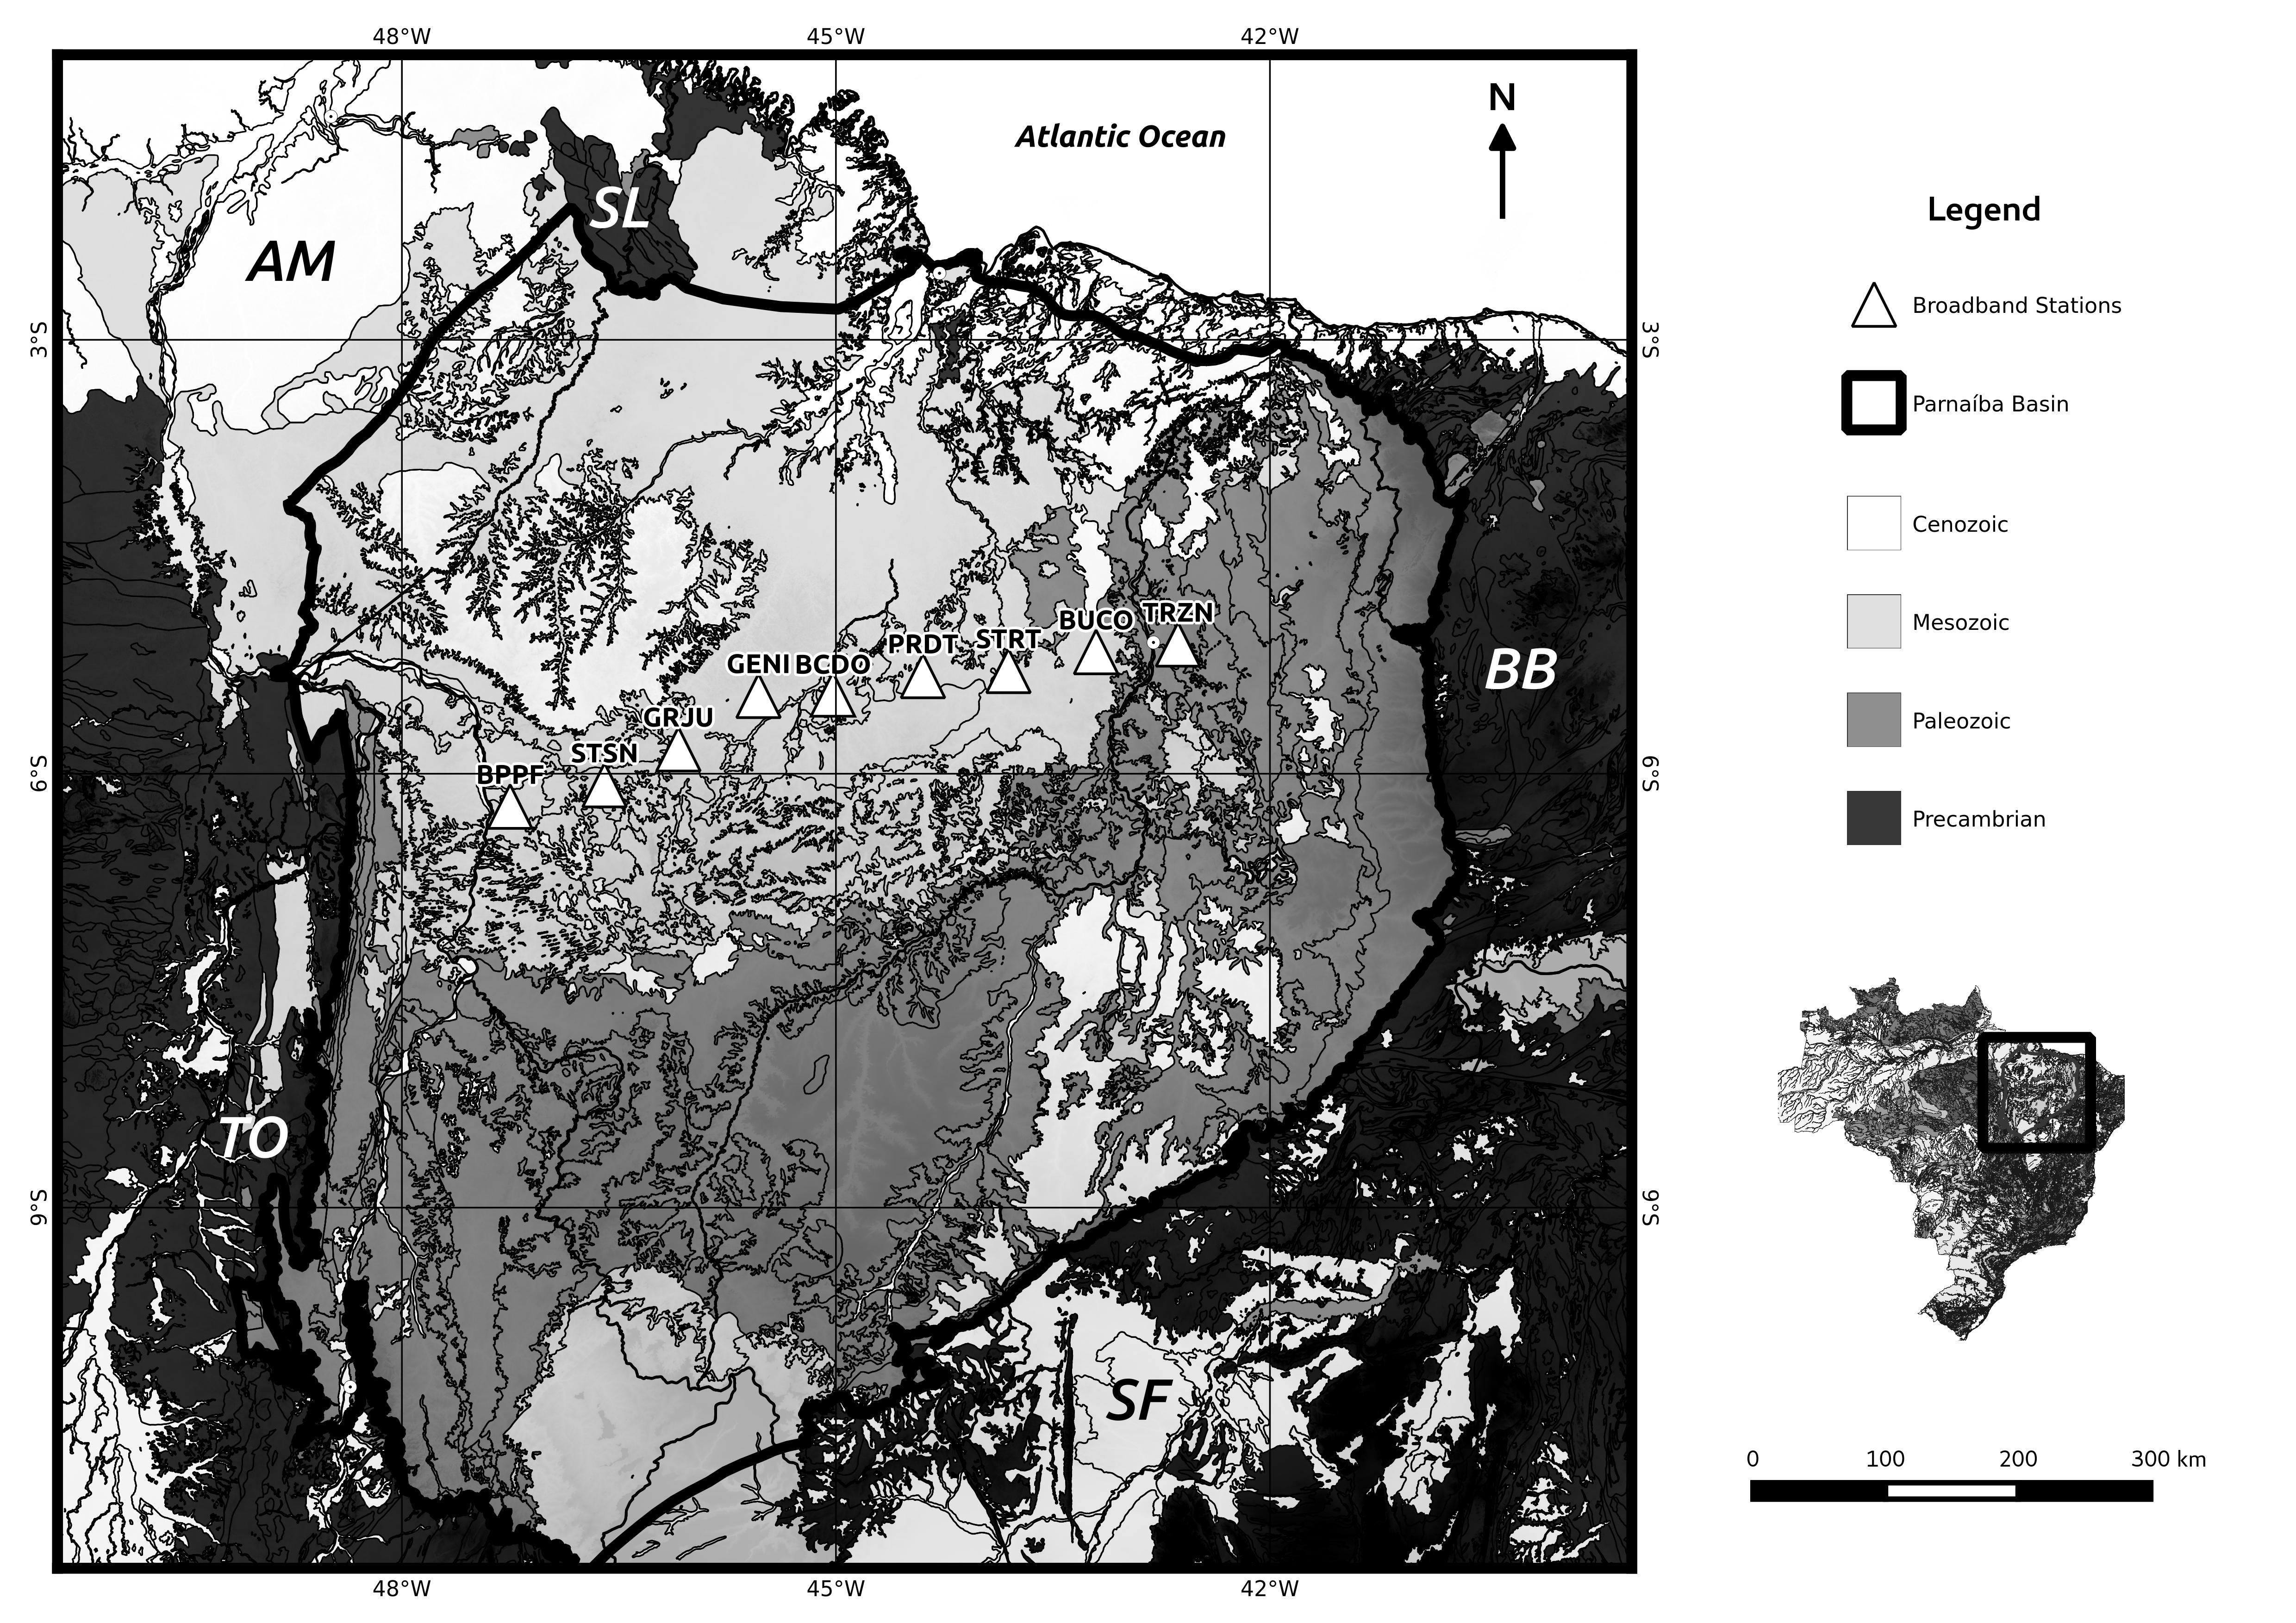
\includegraphics[width=\textwidth]{Fig/Mapa_geologico_BP_grey.pdf}
\caption{Geological map of the Parna\'{\i}ba basin displaying the location of Parna\'{\i}ba Basin Analysis Project (PBAP) stations (triangles) utilized in this study. AM - Amazonian Craton; BB - Borborema Province; SF - S\~ao Francisco Craton; SL - S\~ao Lu\'{\i}s Craton; TO - Tocantins Province.}
\label{mapa_estacoes_geologico}
\end{center}
\end{figure}


\begin{figure}[!ht]
\begin{center}
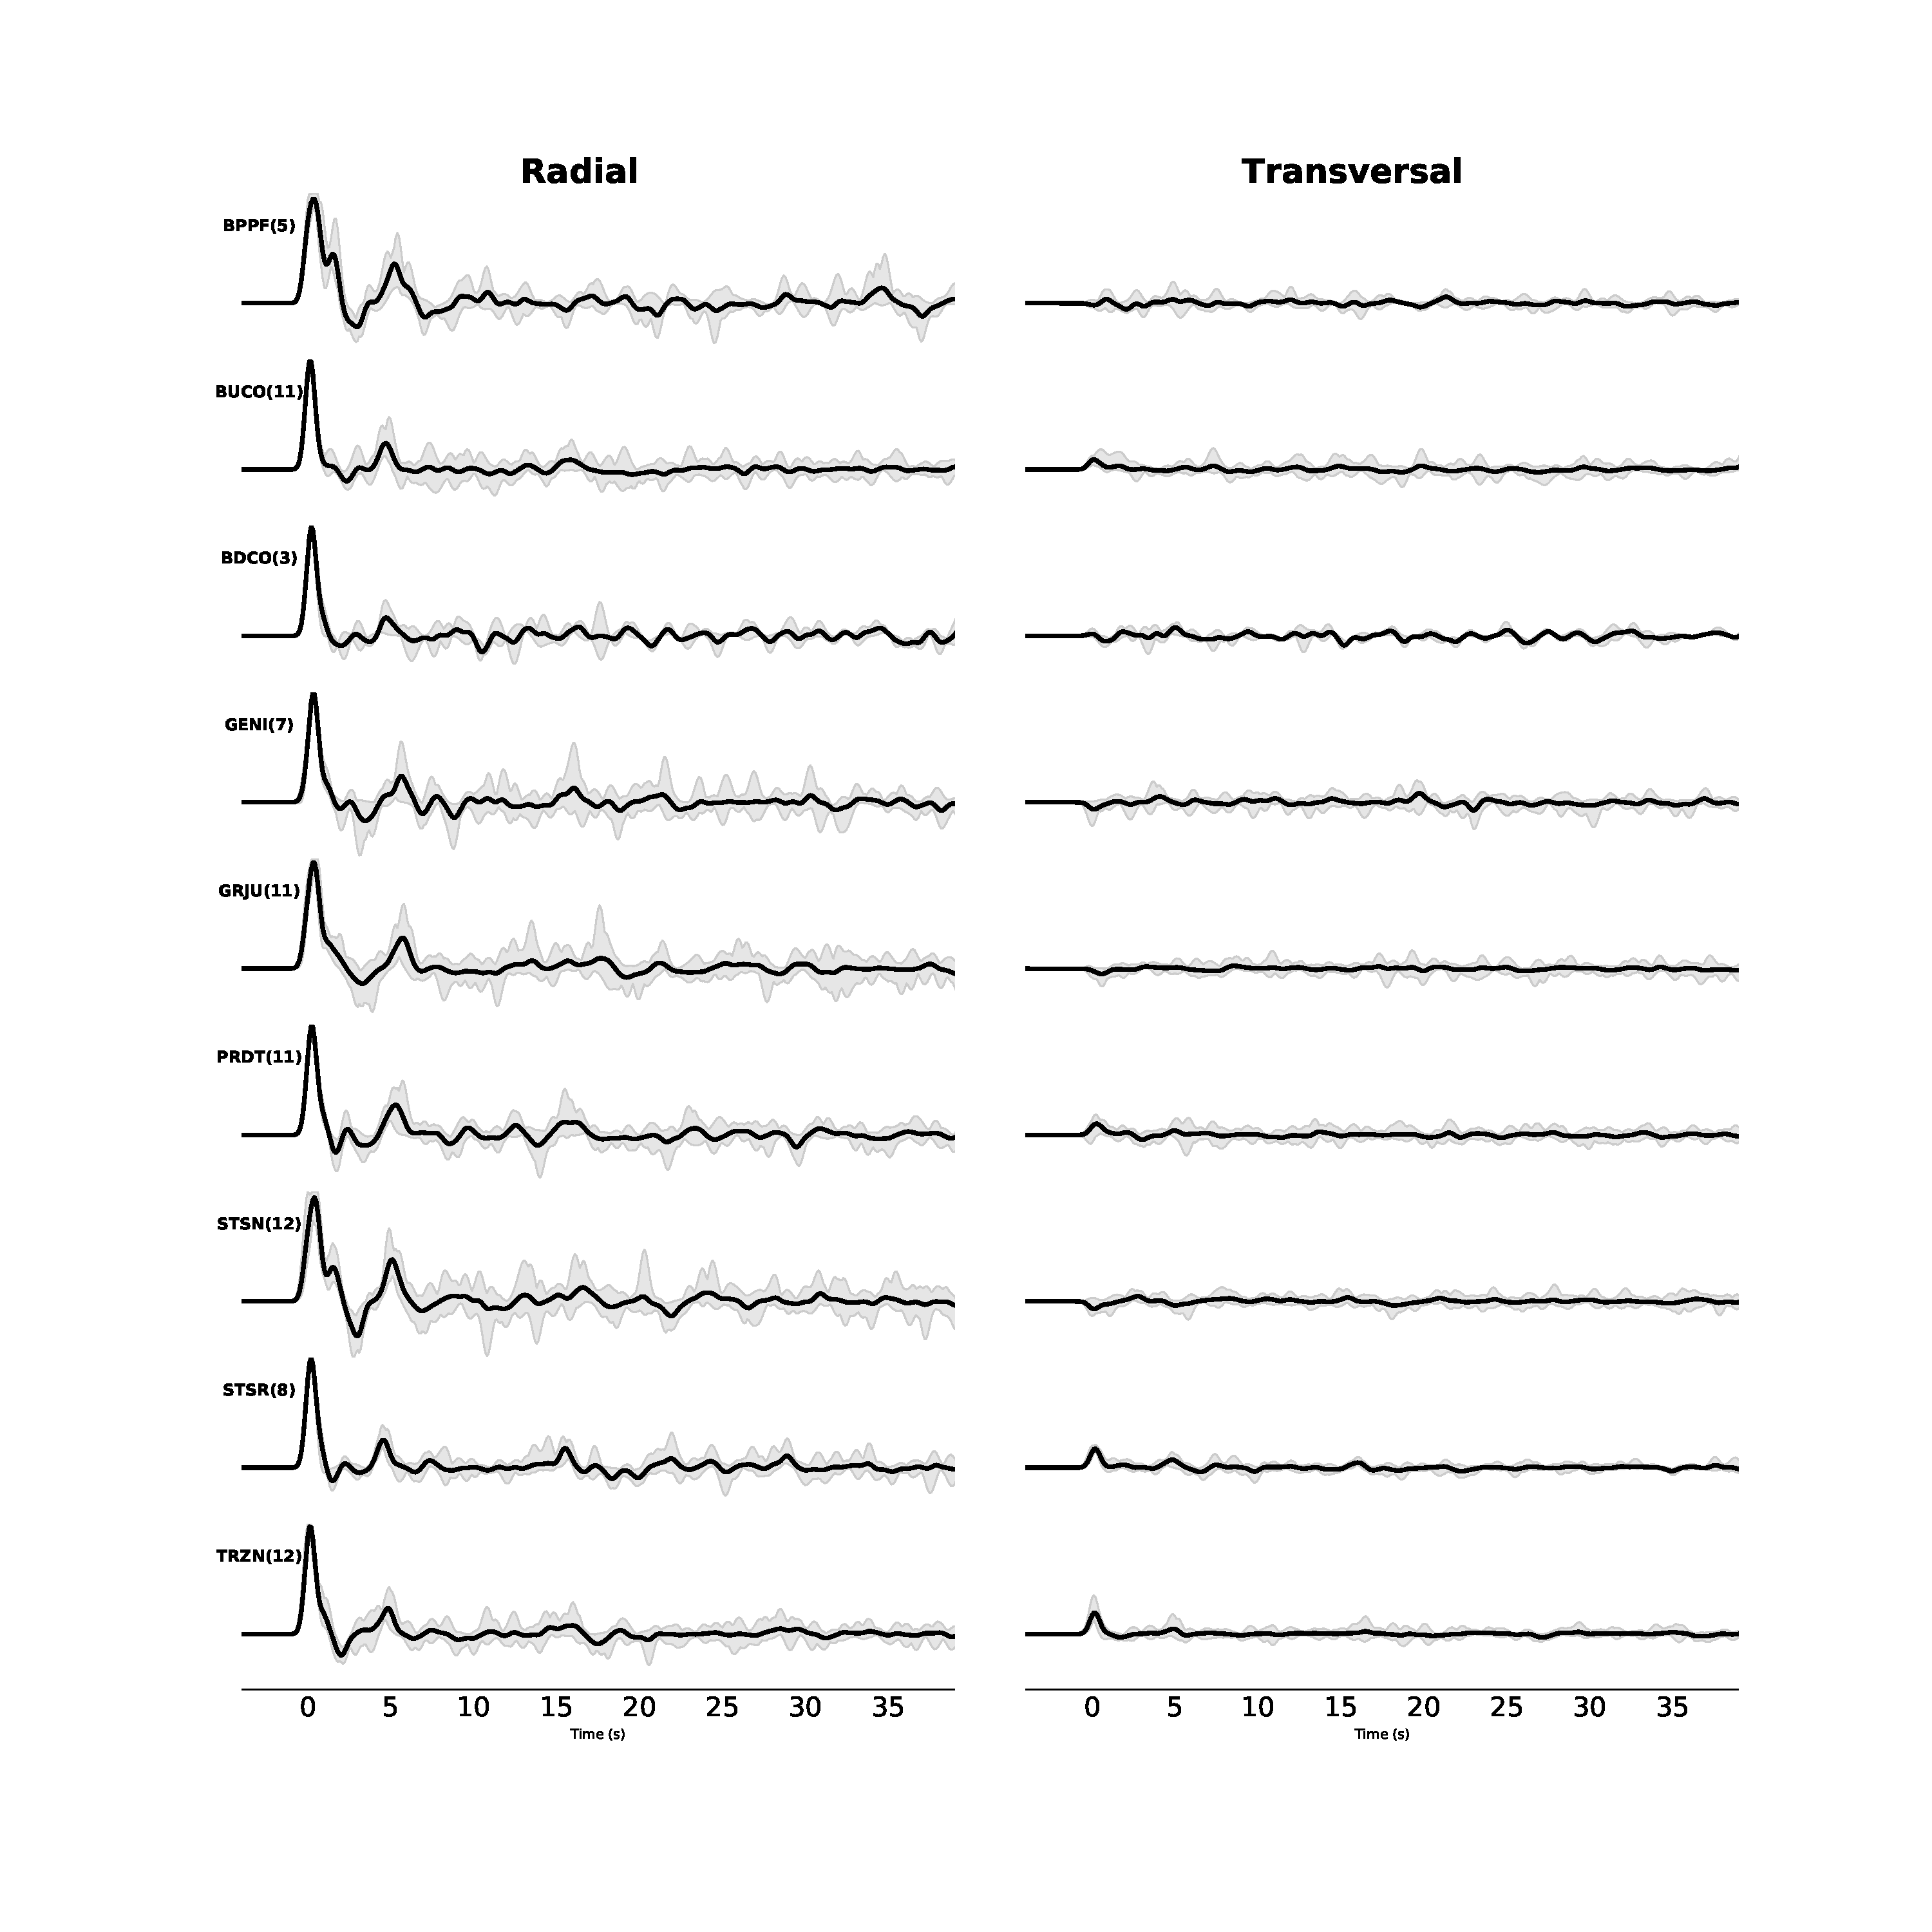
\includegraphics[width=\textwidth]{Fig/stations_FR.pdf}
\caption{Receiver function stacks developed for the seismic stations in the Parna\'{\i}ba basin. Right and left panels refer to radial and transversal receiver functions, respectively. The number of waveforms included in the stack are displayed nest to the station name in the upper left corner of each panel. The stacks are presented through a black line within a gray shade representing 1$\sigma$-confidence bounds for the stacked amplitudes. Although the signature of the sedimentary layers is apparent in the first 3-4 s of the waveforms, it does not seem to interfere with the Ps conversion at $\sim$5 s from the crust-mantle boundary.}
\label{estations_FR}
\end{center}
\end{figure}

\begin{figure}[!ht]
\begin{center}
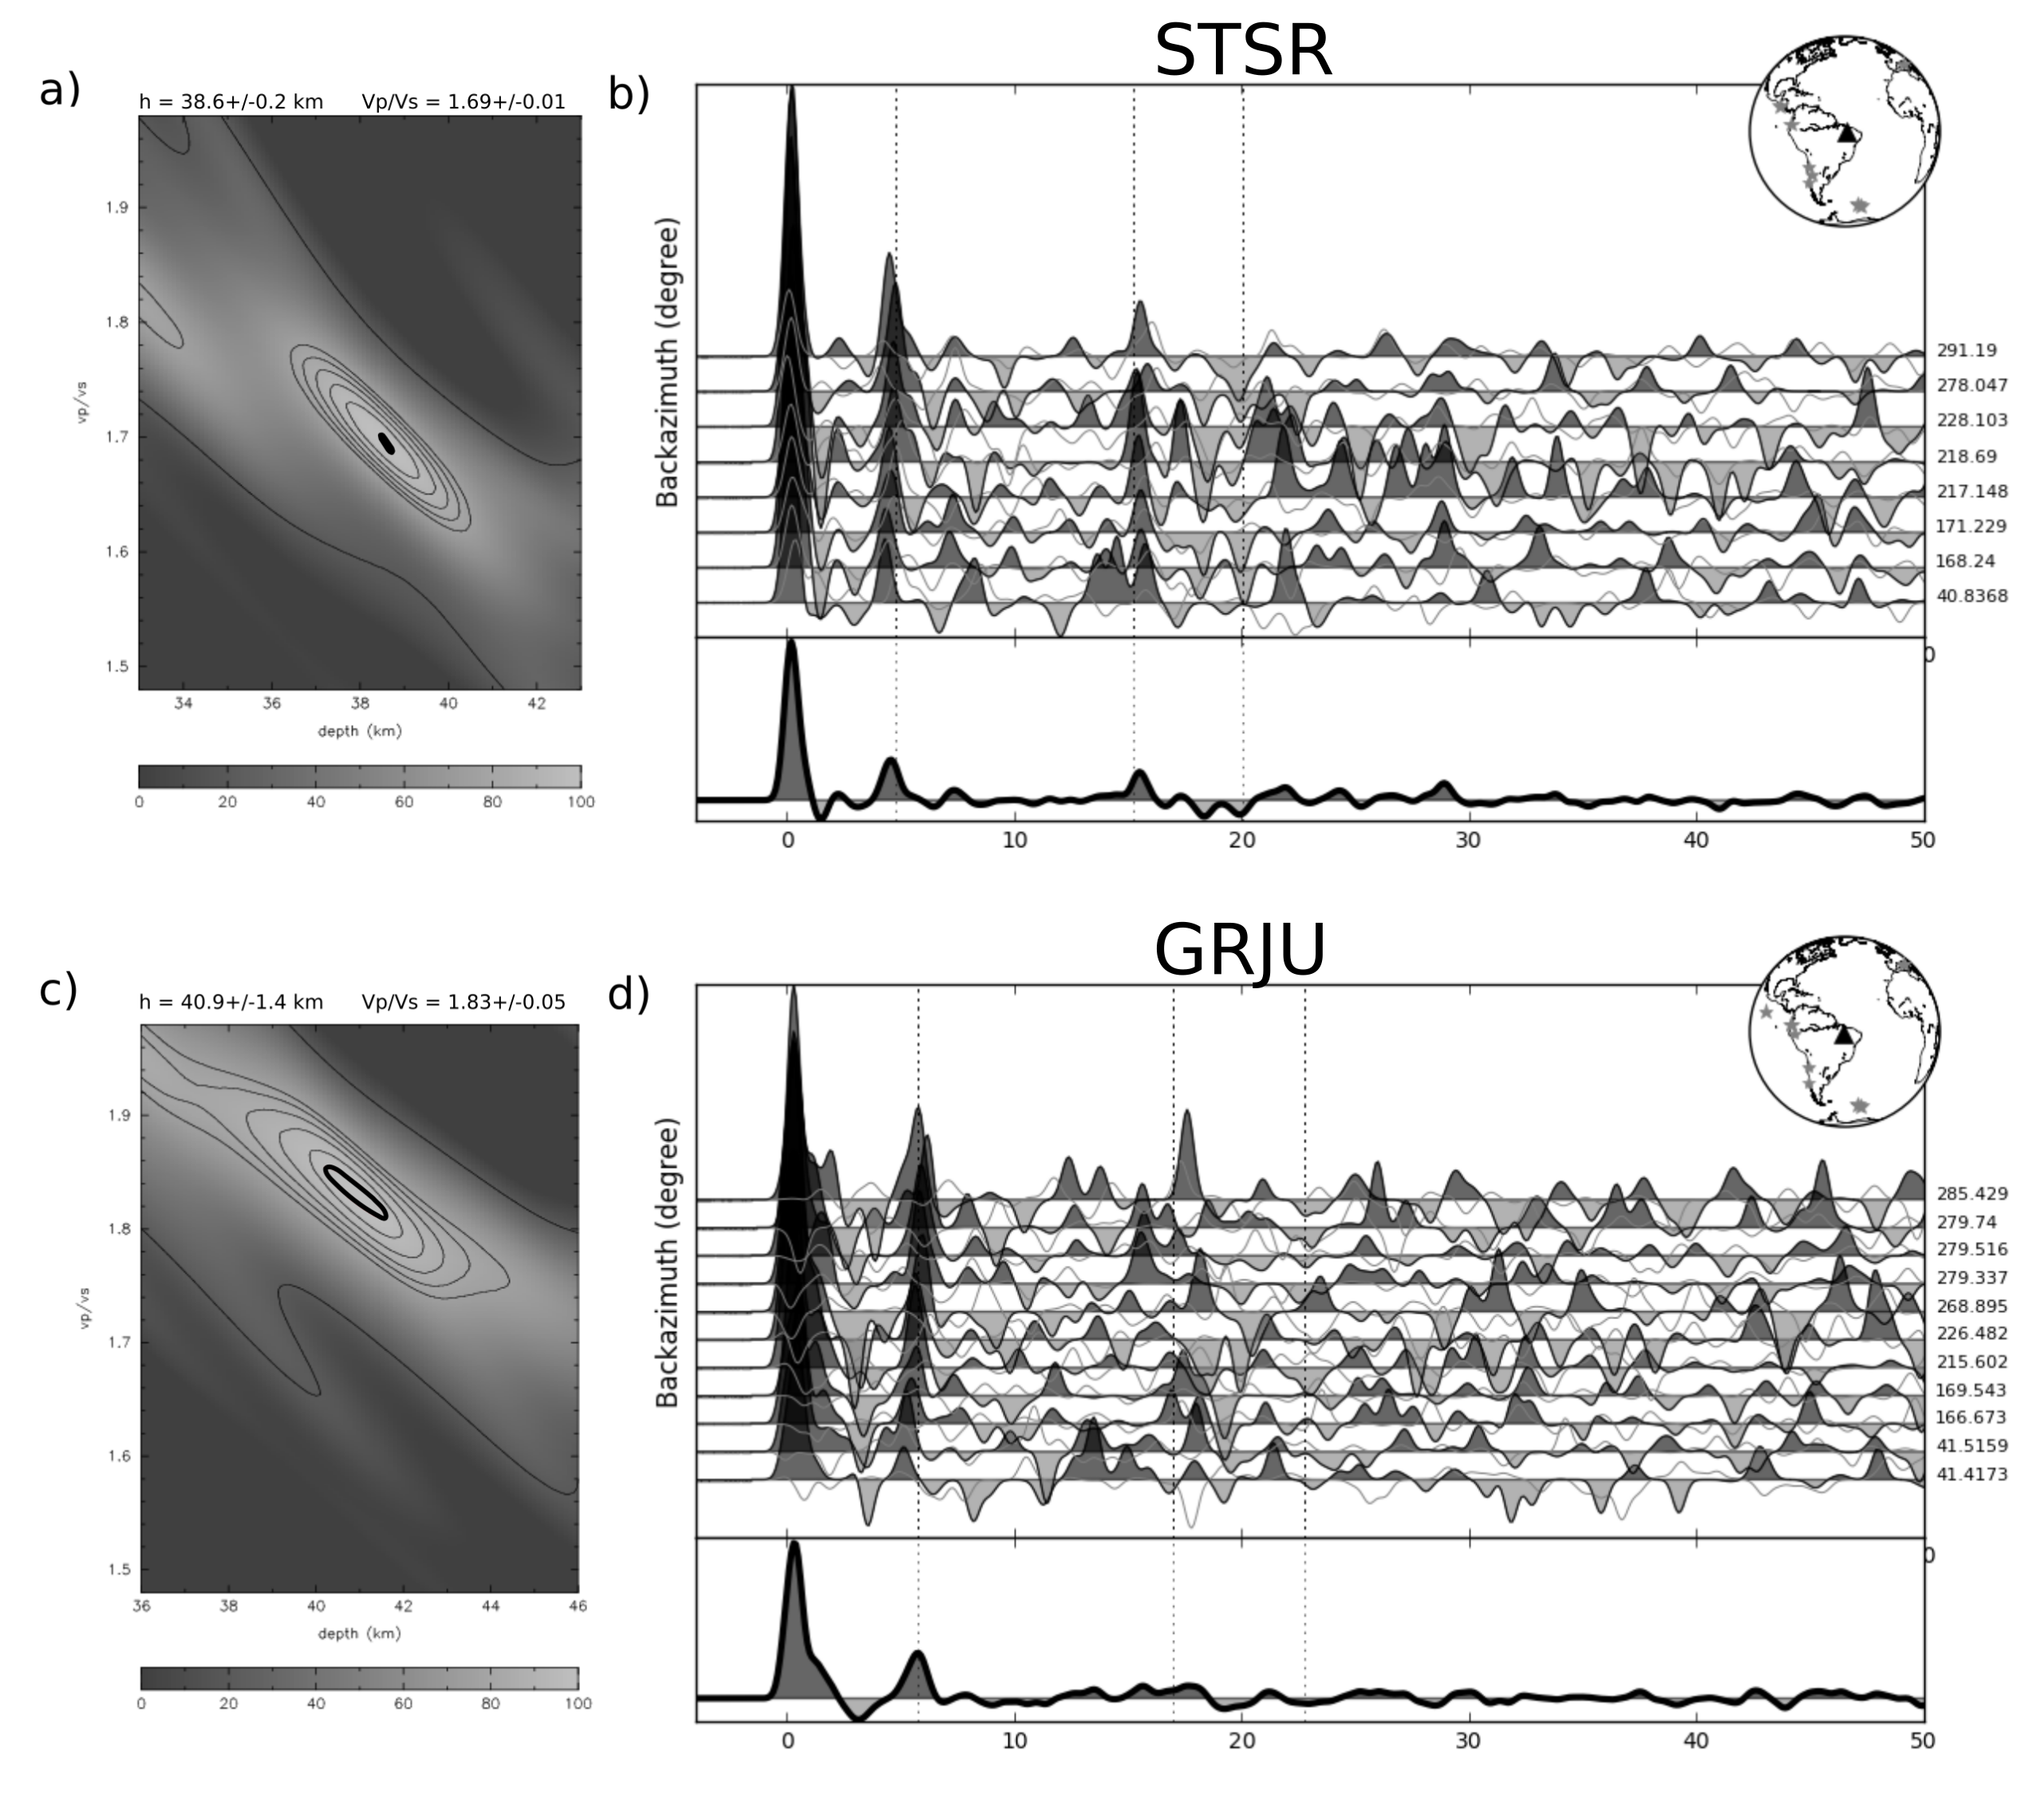
\includegraphics[width=\textwidth]{Fig/mosaico_GRJU_STSR.png}
\caption{Sample H-$\kappa$ stacking results for station STSR and GRJU. The left panels display the H$\kappa$ stacking surfaces, while the right panels display the corresponding radial receiver functions utilized during the stacking procedure. Receiver functions in the right panels were sorted by ray parameter. The thick, black line in panels (a) and (c) is the 1$\sigma$-confidence ellipse from bootstrapping, and the thin, dotted lines in panels (b) and (d) are the phase moveout curves for the Ps, PpPs and PpSs+PsPs phases associated to the maximum in the H$\kappa$-stacking surface. Note the lack of a consistent PpPs multiple at station GRJU and the correspondingly large uncertainties in the resulting crustal thickness and Vp/Vs ratio.
}
\label{moisaic_FR}
\end{center}
\end{figure}

\begin{figure}[!ht]
\begin{center}
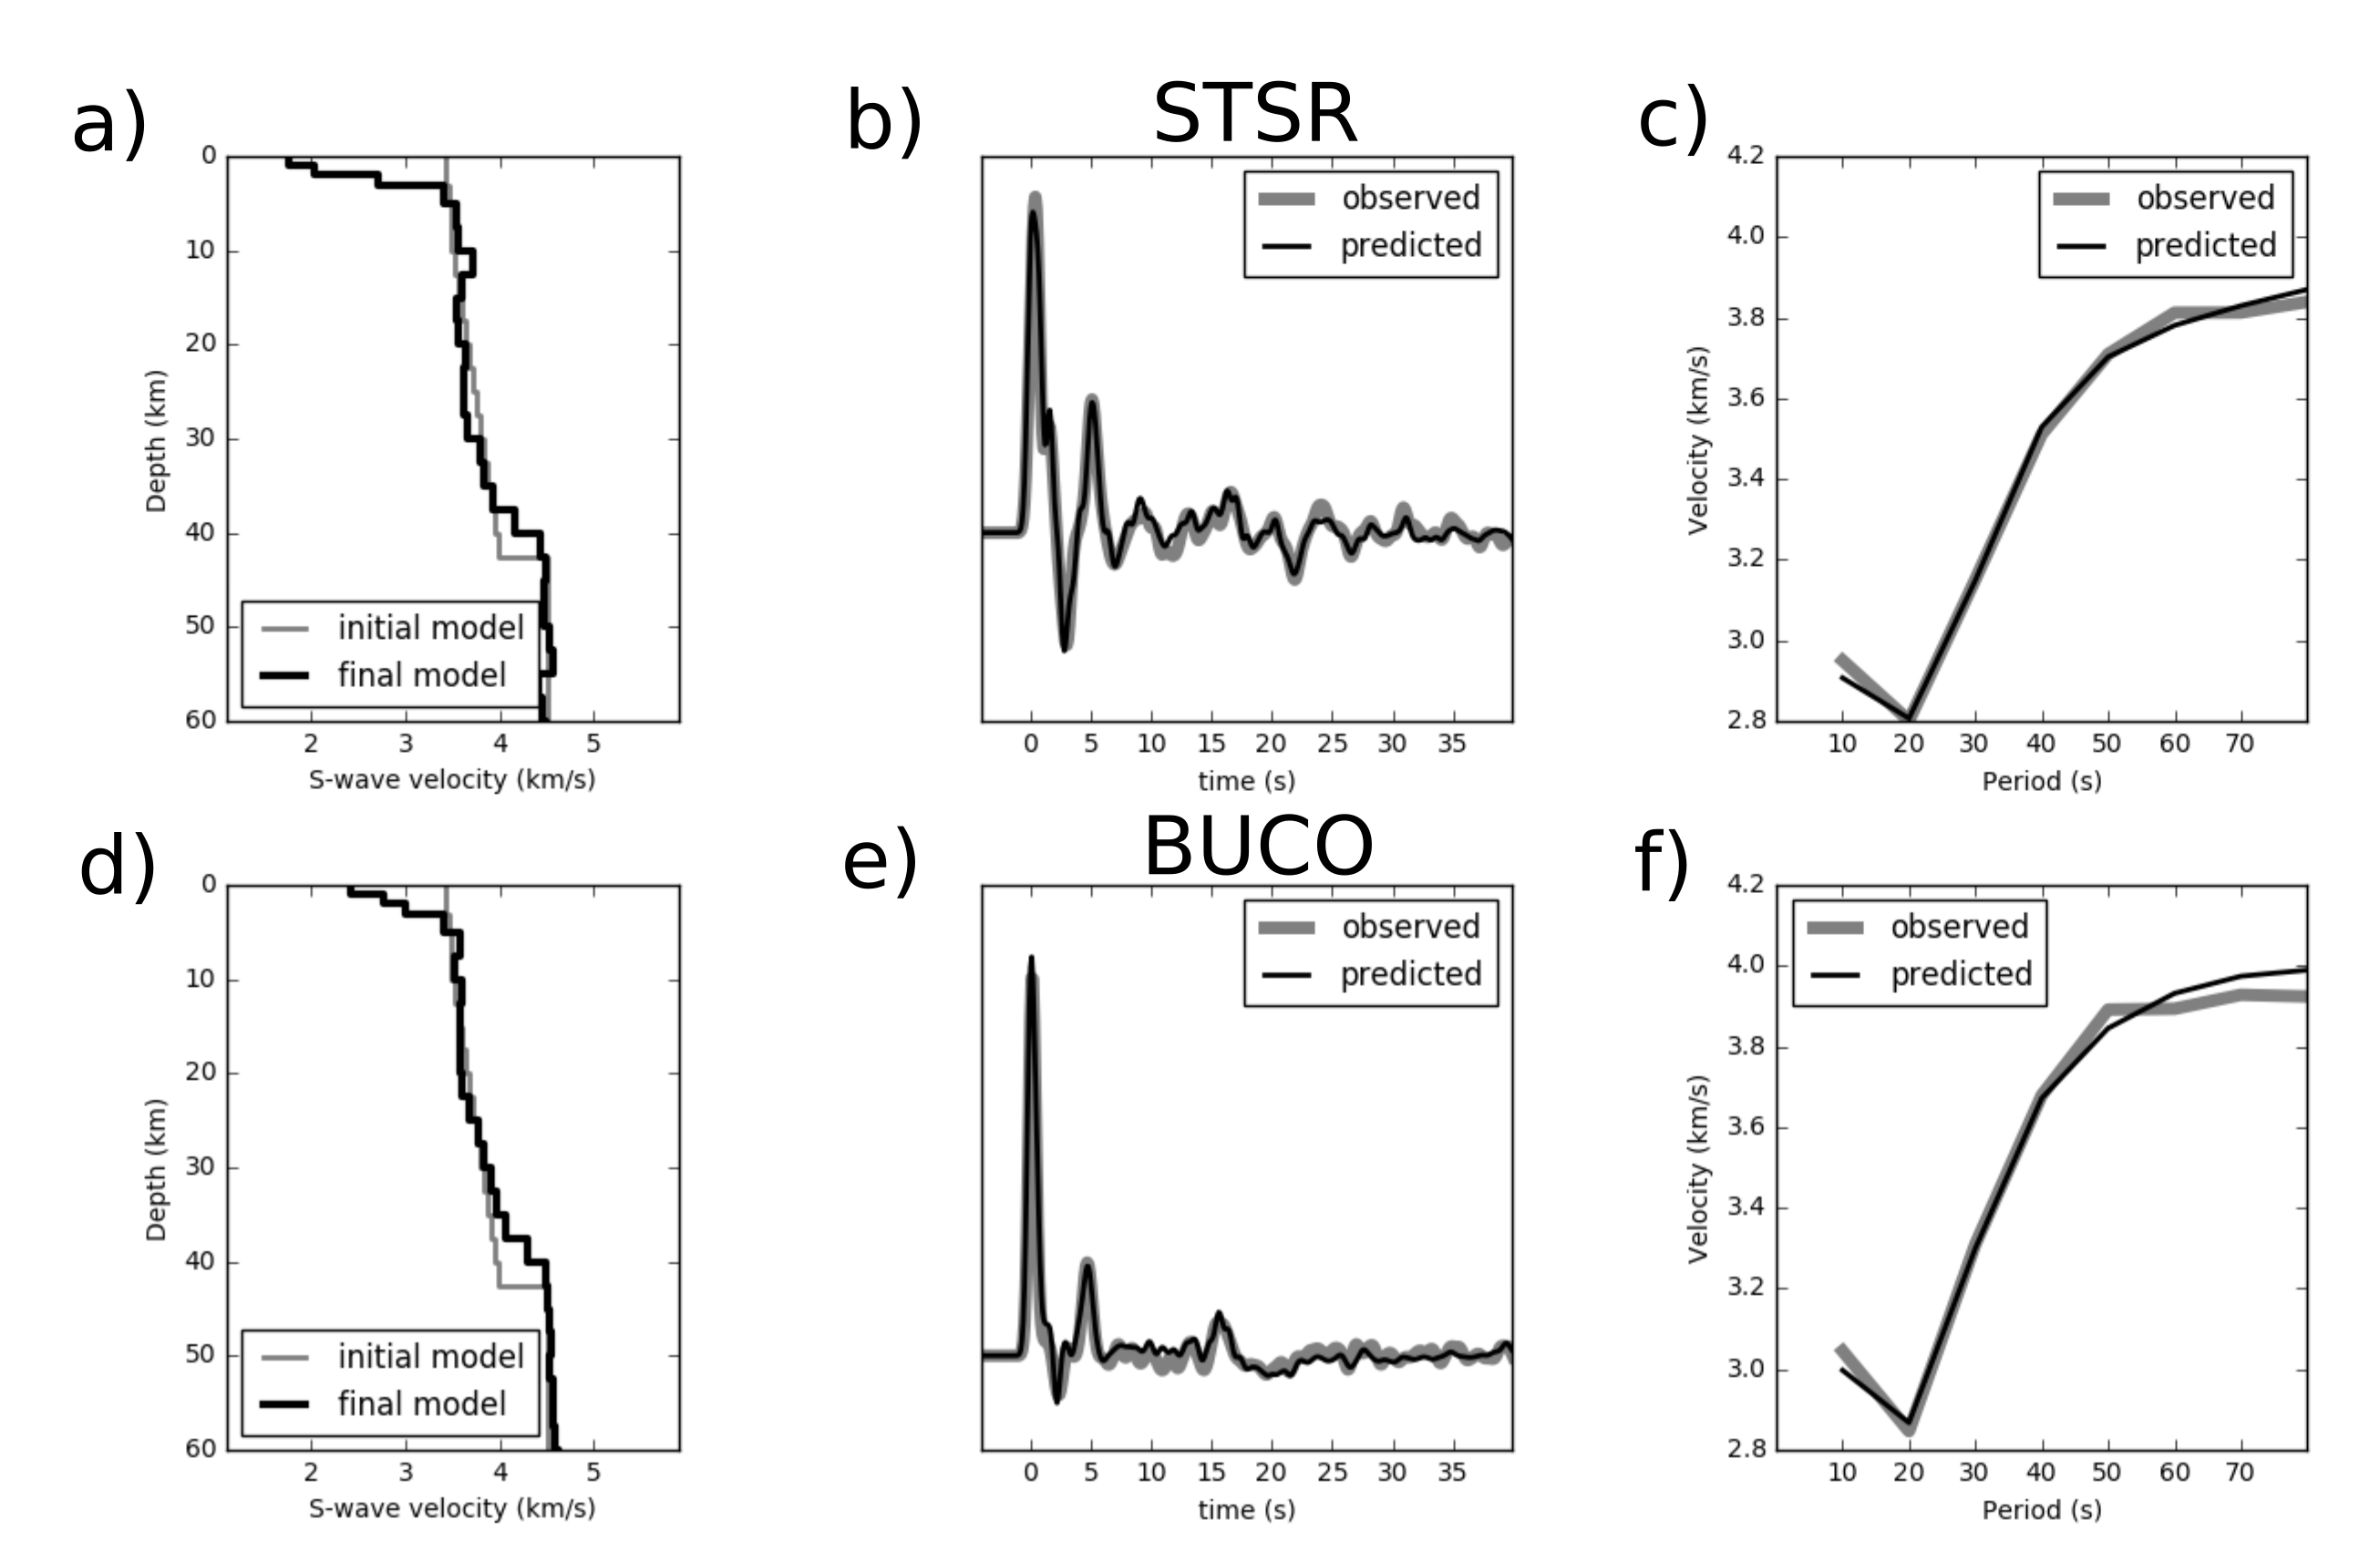
\includegraphics[width=\textwidth]{Fig/joint_inversion_results.png}
\caption{Joint inversion results for statopms STSN and BUCO. The inverted velocity models are shown in the left panels (thick, solid line), along with the starting model utilized in the inversion (thin, solid line). A comparison between observations (gray lines) and predictions (black lines) is given in the middle panels for receiver functions and in the right panels for the dispersion curves. Note the simplicity of the inverted S-velocity profiles and the excellent agreement between observations and predictions, including the large amplitudes in the first 3-4 s in the receiver functions associated to sedimentary structure.}
\label{joint_inversion}
\end{center}
\end{figure}

\begin{figure}[!ht]
\begin{center}
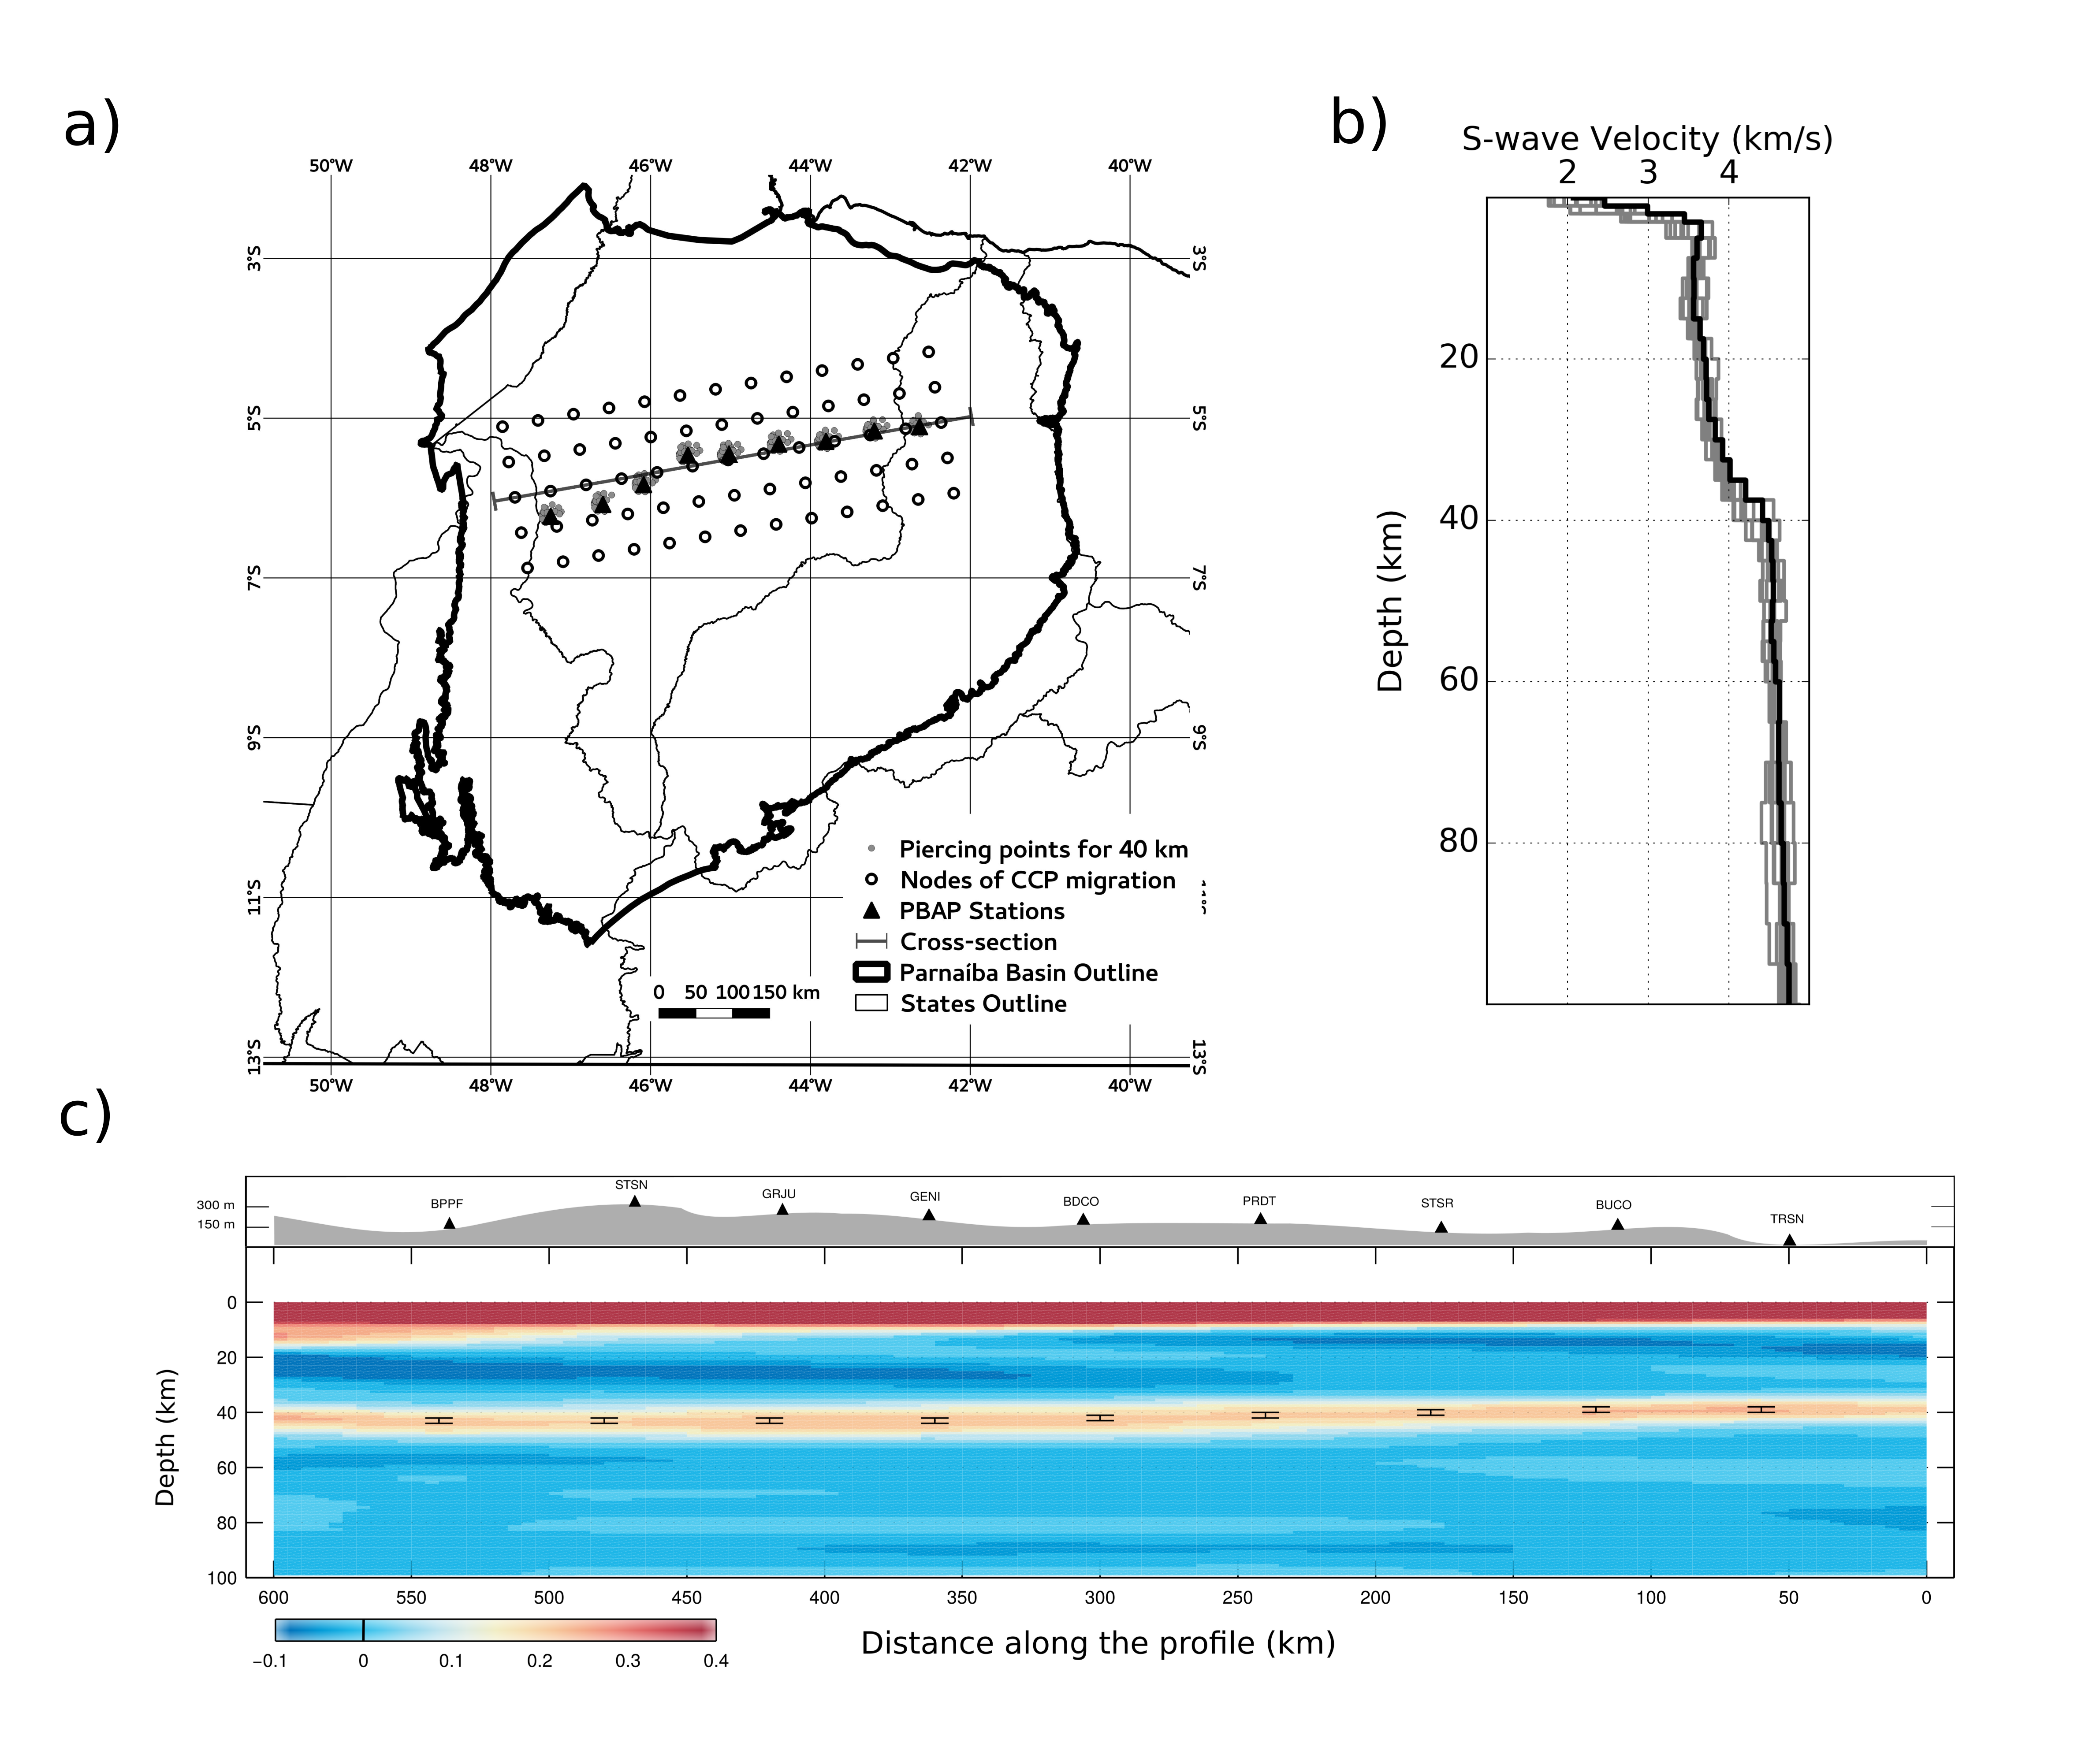
\includegraphics[width=\textwidth]{Fig/section_migration.png}
\caption{Common Conversion Point stacking results for the Parna\'{\i}ba basin. (a) Map showing the locations of seismic stations (black triangles), nodes considered for the CCP stacking (open circles), and CCP profile (black line); (b) Average S-wave velocity model utilized for migration (back-projection) of the receiver functions; and, (c) CCP stack cross-section displaying stacked receiver function amplitudes, where red colors indicate positive amplitudes (i.e. positive velocity contrast), and blue colors indicate negative amplitudes (i.e. negative velocity contrast). The black marks at $\sim$40~km depth are Moho depths estimates obtained from bootstrapping the receiver functions associated to each node along the cross-section. Location of the stations are show on top, superimposed with basin topography.}
\label{moisaic_migration}
\end{center}
\end{figure}

\begin{figure}[!ht]
\begin{center}
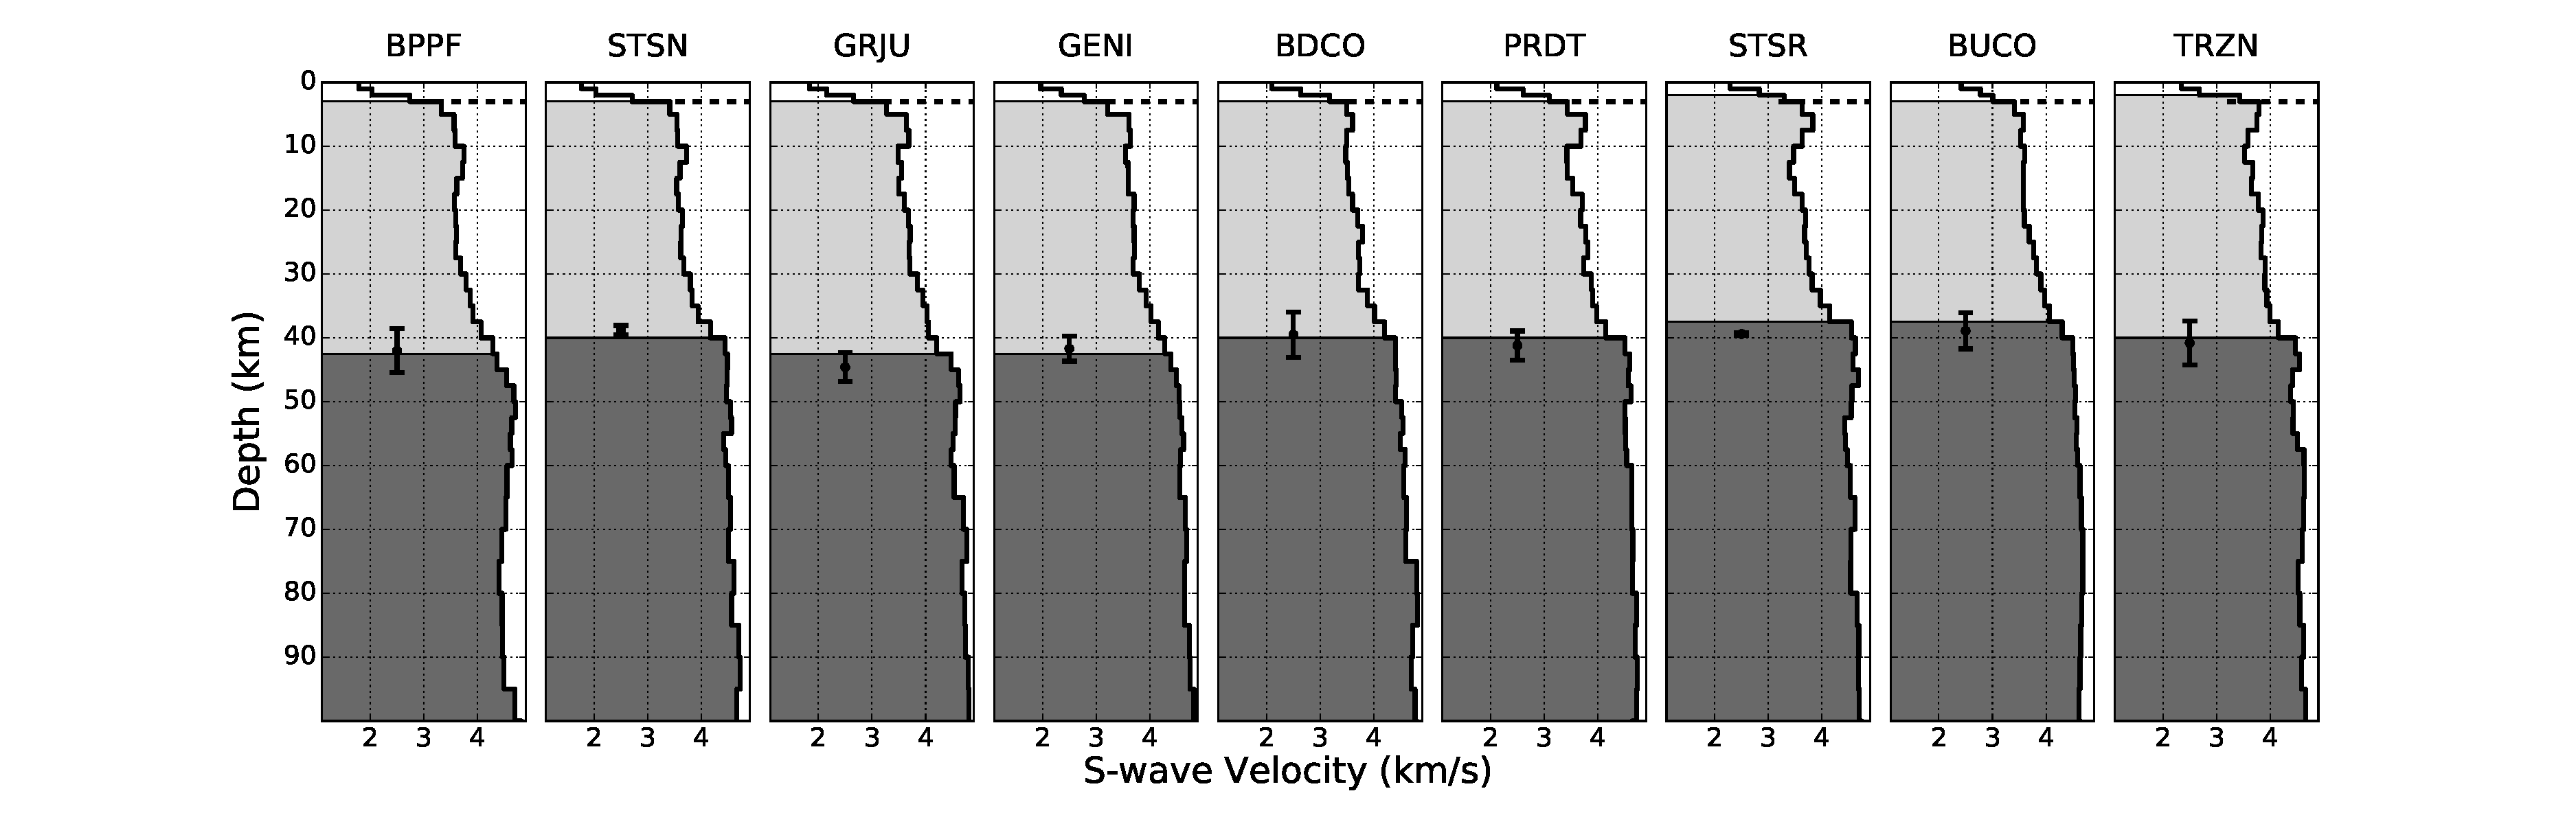
\includegraphics[width=1.1\textwidth]{Fig/section_joint_inversion_25.pdf}
\caption{Joint inversion S-velocity models for each station along the profile, sorted according to station location. The models have been shaded according to velocity to display the main layers: sedimentary layer (Vs $<$ 3.2 km/s) in white; crust (3.2 $<$ Vs $<$ 4.3 km/s) in light gray; and mantle (Vs $>$ 4.3 km/s) in dark gray. Dashed line is placed at 3 km depth. H-$\kappa$ stacking results for crustal thickness are superimposed as vertical lines scaled according to confidence bounds, for comparison. Note the excellent agreement in crustal thickness estimates.}
\label{moisaic_joint_inversion}
\end{center}
\end{figure}
 
\end{document}
